\documentclass[6pt]{article}
\usepackage[margin=1.7cm, a2paper]{geometry}
% \documentclass[border=5pt]{standalone}
\usepackage[usenames,dvipsnames]{xcolor}
\usepackage{float}
\usepackage{tikz}
\usepackage{verbatim}
\usepackage{caption}
\usepackage{pgfplots}
\usepackage{fancyhdr}
\usepackage{lscape}

\pagestyle{fancy}
\rfoot{Written by Sebastien ROUX \copyright 2013 - Eurecom}

% Generate PDF with pdflatex command

\author{Sebastien ROUX}

\usetikzlibrary{calc,trees,positioning,arrows,chains,shapes.geometric,%
    decorations.pathreplacing,decorations.pathmorphing,shapes,%
    matrix,shapes.symbols,backgrounds,fit}

\tikzset{
  background/.style={
      draw,
      fill=yellow!30,
      align=right,
      dashed,
  },
  backgroundcomment/.style={
      draw,
      fill=yellow!30,
      dashed,
  },
  backgroundopt/.style={
      draw,
      fill=blue!2,
      dashed
  },
  schritt/.style={
      draw,
      rounded corners,
      fill=blue!20,
      inner xsep=2em,
  },
  type/.style={
    dashed
  },
  square matrix/.style={
      matrix of nodes,
      draw,
      column sep=-3.5cm, row sep=0.4cm,
      nodes={
%         minimum height=#1,
        anchor=west,
        text width=#1,
        align=left,
        inner sep=0pt
      },
  },
  square matrix/.default=5.5cm
}

% Returns three nodes: The argument, and the projections of the argument on the left and right borders of the bounding box
\newcommand{\extendnode}[1]{
    (#1)
    ($(current bounding box.north east)!(#1)!(current bounding box.south east) + (4.5,0)$)
    ($(current bounding box.north west)!(#1)!(current bounding box.south west)$)
}

\newcommand{\soneapcolor}[1]{
%     {\color{red} #1}
    \color{YellowOrange}{#1}
}
\newcommand{\nascolor}[1]{
%     {\color{red} #1}
    \color{Cyan}{#1}
}
\newcommand{\sctpcolor}[1]{
%     {\color{red} #1}
    \color{LimeGreen}{#1}
}
\newcommand{\ssixcolor}[1]{
%     {\color{red} #1}
    \color{RawSienna}{#1}
}
\newcommand{\mmecolor}[1]{
%     {\color{red} #1}
    \color{Red}{#1}
}
\newcommand{\spappcolor}[1]{
%     {\color{red} #1}
    \color{Mulberry}{#1}
}
\newcommand{\commandname}[1]{
    \large{#1}
}

% argument #1: any options
\newenvironment{customlegend}[1][]{%
    \begingroup
    % inits/clears the lists (which might be populated from previous
    % axes):
    \csname pgfplots@init@cleared@structures\endcsname
    \pgfplotsset{#1}%
}{%
    % draws the legend:
    \csname pgfplots@createlegend\endcsname
    \endgroup
}%

% definition to insert numbers
\pgfkeys{/pgfplots/number in legend/.style={%
/pgfplots/legend image code/.code={%
\node at (0.295,-0.0225){#1};
},%
},
}

% makes \addlegendimage available (typically only available within an
% axis environment):
\def\addlegendimage{\csname pgfplots@addlegendimage\endcsname}

\begin{document}
\begin{center}
\begin{figure}[H]
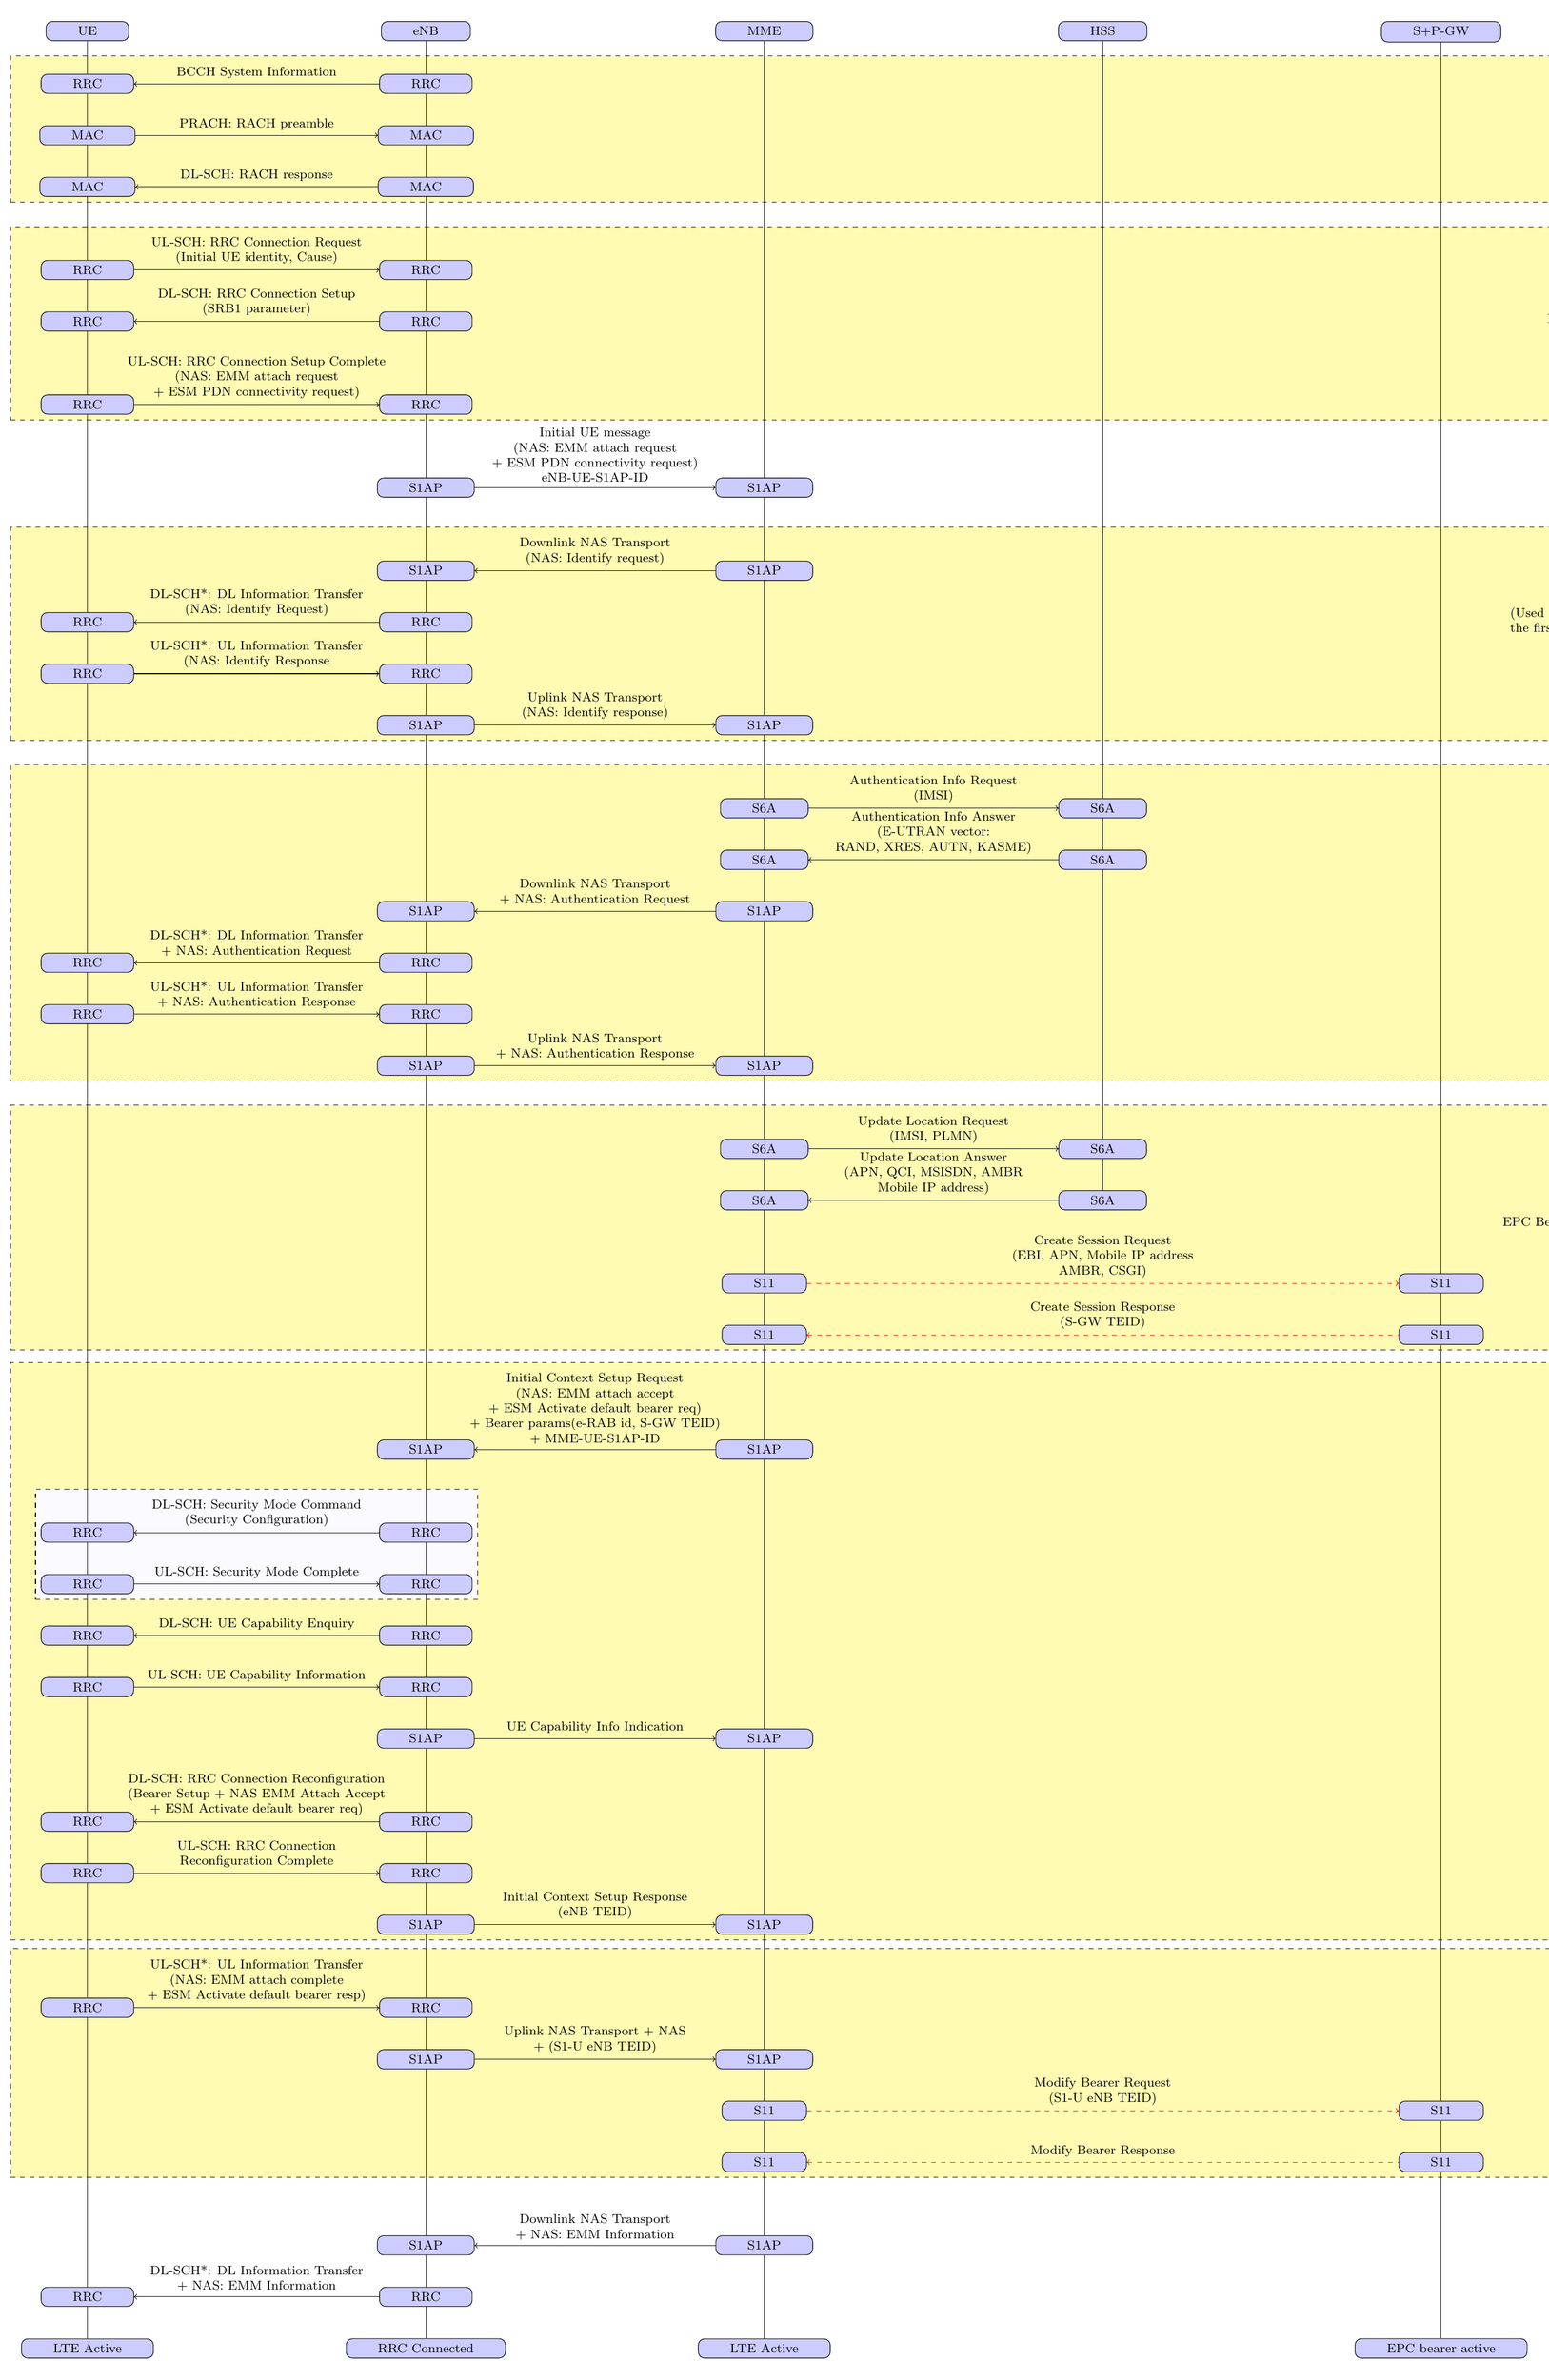
\begin{tikzpicture}
\tikzstyle{every node}=[font=\footnotesize]
\matrix (matrix) [row sep=0.7cm, column sep={7.5cm,between origins}, matrix of nodes] {
    \node(UE) [schritt] {UE}; & \node(ENB) [schritt] {eNB}; & \node(MME) [schritt] {MME}; & \node(HSS) [schritt] {HSS}; & \node(SPGW) [schritt] {S+P-GW};\\
        \node(RRC1UE)   [schritt] {RRC};  & \node(RRC1ENB)   [schritt] {RRC};           \\
        \node(MAC1UE)   [schritt] {MAC};  & \node(MAC1ENB)   [schritt] {MAC};           \\
        \node(MAC2UE)   [schritt] {MAC};  & \node(MAC2ENB)   [schritt] {MAC};           \\\\
        \node(RRC2UE)   [schritt] {RRC};  & \node(RRC2ENB)   [schritt] {RRC};           \\
        \node(RRC3UE)   [schritt] {RRC};  & \node(RRC3ENB)   [schritt] {RRC};           \\\\
        \node(RRC4UE)   [schritt] {RRC};  & \node(RRC4ENB)   [schritt] {RRC};           \\\\
                                          & \node(S1AP1ENB)  [schritt] {S1AP}; & \node(S1AP1MME) [schritt] {S1AP};      \\\\
                                          & \node(S1AP9ENB)  [schritt] {S1AP}; & \node(S1AP9MME) [schritt] {S1AP};      \\
        \node(RRC15UE)  [schritt] {RRC};  & \node(RRC15ENB)  [schritt] {RRC};                                           \\
        \node(RRC16UE)  [schritt] {RRC};  & \node(RRC16ENB)  [schritt] {RRC};                                           \\
                                          & \node(S1AP10ENB) [schritt] {S1AP}; & \node(S1AP10MME) [schritt] {S1AP};     \\\\
                                          &                                    & \node(S6A1MME) [schritt] {S6A};        & \node(S6A1HSS) [schritt] {S6A};\\
                                          &                                    & \node(S6A2MME) [schritt] {S6A};        & \node(S6A2HSS) [schritt] {S6A};\\
                                          & \node(S1AP6ENB)  [schritt] {S1AP}; & \node(S1AP6MME) [schritt] {S1AP}; \\
        \node(RRC11UE)  [schritt] {RRC};  & \node(RRC11ENB)  [schritt] {RRC};           \\
        \node(RRC12UE)  [schritt] {RRC};  & \node(RRC12ENB)  [schritt] {RRC};           \\
                                          & \node(S1AP7ENB)  [schritt] {S1AP}; & \node(S1AP7MME) [schritt] {S1AP}; \\\\
                                          &                                    & \node(S6A3MME) [schritt] {S6A};        & \node(S6A3HSS) [schritt] {S6A};\\
                                          &                                    & \node(S6A4MME) [schritt] {S6A};        & \node(S6A4HSS) [schritt] {S6A};\\\\
                                          &                                    & \node(S11MME1)  [schritt] {S11};       &       & \node(S11SPGW1) [schritt] {S11}; \\
                                          &                                    & \node(S11MME2)  [schritt] {S11};       &       & \node(S11SPGW2) [schritt] {S11}; \\\\\\
                                          & \node(S1AP2ENB) [schritt] {S1AP};  & \node(S1AP2MME) [schritt] {S1AP}; \\\\
        \node(RRC5UE)   [schritt] {RRC};  & \node(RRC5ENB)  [schritt] {RRC};            \\
        \node(RRC6UE)   [schritt] {RRC};  & \node(RRC6ENB)  [schritt] {RRC};            \\
        \node(RRC13UE)  [schritt] {RRC};  & \node(RRC13ENB)  [schritt] {RRC};           \\
        \node(RRC14UE)  [schritt] {RRC};  & \node(RRC14ENB)  [schritt] {RRC};           \\
                                          & \node(S1AP8ENB) [schritt] {S1AP};  & \node(S1AP8MME) [schritt] {S1AP}; \\\\
        \node(RRC7UE)   [schritt] {RRC};  & \node(RRC7ENB)  [schritt] {RRC};            \\
        \node(RRC8UE)   [schritt] {RRC};  & \node(RRC8ENB)  [schritt] {RRC};            \\
                                          & \node(S1AP3ENB) [schritt] {S1AP};  & \node(S1AP3MME) [schritt] {S1AP}; \\\\
        \node(RRC9UE)   [schritt] {RRC};  & \node(RRC9ENB)  [schritt] {RRC};            \\
                                          & \node(S1AP4ENB) [schritt] {S1AP};  & \node(S1AP4MME) [schritt] {S1AP}; \\
                                          &                                    & \node(S11MME3)  [schritt] {S11};       &       & \node(S11SPGW3) [schritt] {S11}; \\
                                          &                                    & \node(S11MME4)  [schritt] {S11};       &       & \node(S11SPGW4) [schritt] {S11}; \\\\
                                          & \node(S1AP5ENB) [schritt] {S1AP};  & \node(S1AP5MME) [schritt] {S1AP}; \\
        \node(RRC10UE)   [schritt] {RRC}; & \node(RRC10ENB)  [schritt] {RRC};           \\
        \node(UELTEACTIVE)[schritt] {LTE Active}; & \node(RRCCONNECTED) [schritt] {RRC Connected}; & \node(MMELTEACTIVE) [schritt] {LTE Active}; & & \node(BEARERCREATED) [schritt] {EPC bearer active};\\
    };

    \draw[<-] (node cs:name=RRC1UE,anchor=east)    -- node(arrow1) [above, align=center]{BCCH System Information}(node cs:name=RRC1ENB,anchor=west);
    \draw[->] (node cs:name=MAC1UE,anchor=east)    -- node         [above, align=center]{PRACH: RACH preamble}(node cs:name=MAC1ENB,anchor=west);
    \draw[<-] (node cs:name=MAC2UE,anchor=east)    -- node         [above, align=center]{DL-SCH: RACH response}(node cs:name=MAC2ENB,anchor=west);
    \draw[->] (node cs:name=RRC2UE,anchor=east)    -- node(arrow2) [above, align=center]{UL-SCH: RRC Connection Request\\(Initial UE identity, Cause)}(node cs:name=RRC2ENB,anchor=west);
    \draw[<-] (node cs:name=RRC3UE,anchor=east)    -- node         [above, align=center]{DL-SCH: RRC Connection Setup\\(SRB1 parameter)}(node cs:name=RRC3ENB,anchor=west);
    \draw[->] (node cs:name=RRC4UE,anchor=east)    -- node         [above, align=center]{UL-SCH: RRC Connection Setup Complete\\(NAS: EMM attach request\\+ ESM PDN connectivity request)}(node cs:name=RRC4ENB,anchor=west);
    \draw[->] (node cs:name=S1AP1ENB,anchor=east)  -- node         [above, align=center]{Initial UE message\\(NAS: EMM attach request\\+ ESM PDN connectivity request)\\eNB-UE-S1AP-ID}(node cs:name=S1AP1MME,anchor=west);
    \draw[<-] (node cs:name=S1AP9ENB,anchor=east)  -- node(arrow10)[above, align=center]{Downlink NAS Transport\\(NAS: Identify request)}                       (node cs:name=S1AP9MME,anchor=west);
    \draw[<-] (node cs:name=RRC15UE,anchor=east)    -- node(arrow6) [above, align=center]{DL-SCH*: DL Information Transfer\\(NAS: Identify Request)}            (node cs:name=RRC15ENB,anchor=west);
    \draw[->] (node cs:name=RRC16UE,anchor=east)    -- node         [above, align=center]{UL-SCH*: UL Information Transfer\\(NAS: Identify Response}            (node cs:name=RRC16ENB,anchor=west);
    \draw[->] (node cs:name=S1AP10ENB,anchor=east) -- node(arrow11)[above, align=center]{Uplink NAS Transport\\(NAS: Identify response)}                        (node cs:name=S1AP10MME,anchor=west);
    \draw[<-] (node cs:name=S1AP2ENB,anchor=east)  -- node(arrow3) [above, align=center]{Initial Context Setup Request\\(NAS: EMM attach accept\\+ ESM Activate default bearer req)\\+ Bearer params(e-RAB id, S-GW TEID)\\+ MME-UE-S1AP-ID}(node cs:name=S1AP2MME,anchor=west);
    \draw[<-] (node cs:name=RRC5UE,anchor=east)    -- node(arrow6) [above, align=center]{DL-SCH: Security Mode Command\\(Security Configuration)}               (node cs:name=RRC5ENB,anchor=west);
    \draw[->] (node cs:name=RRC6UE,anchor=east)    -- node         [above, align=center]{UL-SCH: Security Mode Complete}(node cs:name=RRC6ENB,anchor=west);
    \draw[<-] (node cs:name=RRC7UE,anchor=east)    -- node         [above, align=center]{DL-SCH: RRC Connection Reconfiguration\\(Bearer Setup + NAS EMM Attach Accept\\+ ESM Activate default bearer req)}(node cs:name=RRC7ENB,anchor=west);
    \draw[->] (node cs:name=RRC8UE,anchor=east)    -- node         [above, align=center]{UL-SCH: RRC Connection \\Reconfiguration Complete}(node cs:name=RRC8ENB,anchor=west);
    \draw[->] (node cs:name=S1AP3ENB,anchor=east)  -- node         [above, align=center]{Initial Context Setup Response\\(eNB TEID)}(node cs:name=S1AP3MME,anchor=west);
    \draw[->] (node cs:name=RRC9UE,anchor=east)    -- node(arrow5) [above, align=center]{UL-SCH*: UL Information Transfer\\(NAS: EMM attach complete\\+ ESM Activate default bearer resp)}(node cs:name=RRC9ENB,anchor=west);
    \draw[->] (node cs:name=S1AP4ENB,anchor=east)  -- node          [above, align=center]{Uplink NAS Transport + NAS\\+ (S1-U eNB TEID)}(node cs:name=S1AP4MME,anchor=west);
    \draw[dashed, draw=red, ->] (node cs:name=S11MME1,anchor=east) -- node(arrow4)[above, align=center]{Create Session Request\\(EBI, APN, Mobile IP address\\AMBR, CSGI)}(node cs:name=S11SPGW1,anchor=west);
    \draw[dashed, draw=red,<-] (node cs:name=S11MME2,anchor=east)  -- node[above, align=center]{Create Session Response\\(S-GW TEID)}(node cs:name=S11SPGW2,anchor=west);
    \draw[dashed, draw=red,->] (node cs:name=S11MME3,anchor=east)  -- node[above, align=center]{Modify Bearer Request\\(S1-U eNB TEID)}(node cs:name=S11SPGW3,anchor=west);
    \draw[dashed, draw=red,<-] (node cs:name=S11MME4,anchor=east)  -- node[above, align=center]{Modify Bearer Response}(node cs:name=S11SPGW4,anchor=west);
    \draw[<-] (node cs:name=RRC10UE,anchor=east)   -- node         [above, align=center]{DL-SCH*: DL Information Transfer\\+ NAS: EMM Information}(node cs:name=RRC10ENB,anchor=west);
    \draw[<-] (node cs:name=S1AP5ENB,anchor=east)  -- node         [above, align=center]{Downlink NAS Transport\\+ NAS: EMM Information}(node cs:name=S1AP5MME,anchor=west);
    \draw[<-] (node cs:name=RRC11UE,anchor=east)   -- node         [above, align=center]{DL-SCH*: DL Information Transfer\\+ NAS: Authentication Request}(node cs:name=RRC11ENB,anchor=west);
    \draw[->] (node cs:name=RRC12UE,anchor=east)   -- node         [above, align=center]{UL-SCH*: UL Information Transfer\\+ NAS: Authentication Response}(node cs:name=RRC12ENB,anchor=west);
    \draw[<-] (node cs:name=S1AP6ENB,anchor=east)  -- node(arrow7) [above, align=center]{Downlink NAS Transport\\+ NAS: Authentication Request}(node cs:name=S1AP6MME,anchor=west);
    \draw[->] (node cs:name=S1AP7ENB,anchor=east)  -- node         [above, align=center]{Uplink NAS Transport\\+ NAS: Authentication Response}(node cs:name=S1AP7MME,anchor=west);
    \draw[<-] (node cs:name=RRC13UE,anchor=east)   -- node         [above, align=center]{DL-SCH: UE Capability Enquiry}(node cs:name=RRC13ENB,anchor=west);
    \draw[->] (node cs:name=RRC14UE,anchor=east)   -- node         [above, align=center]{UL-SCH: UE Capability Information}(node cs:name=RRC14ENB,anchor=west);
    \draw[->] (node cs:name=S1AP8ENB,anchor=east)  -- node         [above, align=center]{UE Capability Info Indication}(node cs:name=S1AP8MME,anchor=west);
    \draw[<-] (node cs:name=S6A4MME,anchor=east)   -- node         [above, align=center]{Update Location Answer\\(APN, QCI, MSISDN, AMBR\\Mobile IP address)}(node cs:name=S6A4HSS,anchor=west);
    \draw[->] (node cs:name=S6A3MME,anchor=east)   -- node(arrow9) [above, align=center]{Update Location Request\\(IMSI, PLMN)}(node cs:name=S6A3HSS,anchor=west);
    \draw[->] (node cs:name=S6A1MME,anchor=east)   -- node(arrow8) [above, align=center]{Authentication Info Request\\(IMSI)}(node cs:name=S6A1HSS,anchor=west);
    \draw[<-] (node cs:name=S6A2MME,anchor=east)   -- node         [above, align=center]{Authentication Info Answer\\(E-UTRAN vector:\\RAND, XRES, AUTN, KASME)}(node cs:name=S6A2HSS,anchor=west);
    \label{as1};

    \path[-]
    (UE)      edge (RRC1UE)
    (RRC1UE)  edge (MAC1UE)
    (MAC1UE)  edge (MAC2UE)
    (MAC2UE)  edge (RRC2UE)
    (RRC2UE)  edge (RRC3UE)
    (RRC3UE)  edge (RRC4UE)
    (RRC4UE)  edge (RRC15UE)
    (RRC15UE) edge (RRC16UE)
    (RRC16UE) edge (RRC11UE)
    (RRC11UE) edge (RRC12UE)
    (RRC12UE) edge (RRC5UE)
    (RRC5UE)  edge (RRC6UE)
    (RRC6UE)  edge (RRC13UE)
    (RRC13UE) edge (RRC14UE)
    (RRC14UE) edge (RRC7UE)
    (RRC7UE)  edge (RRC8UE)
    (RRC8UE)  edge (RRC9UE)
    (RRC9UE)  edge (RRC10UE)
    (RRC10UE) edge (UELTEACTIVE)

    (ENB)      edge (RRC1ENB)
    (RRC1ENB)  edge (MAC1ENB)
    (MAC1ENB)  edge (MAC2ENB)
    (MAC2ENB)  edge (RRC2ENB)
    (RRC2ENB)  edge (RRC3ENB)
    (RRC3ENB)  edge (RRC4ENB)
    (RRC4ENB)  edge (S1AP1ENB)
    (S1AP1ENB) edge (S1AP9ENB)
    (S1AP9ENB) edge (RRC15ENB)
    (RRC15ENB) edge (RRC16ENB)
    (RRC16ENB) edge (S1AP10ENB)
    (S1AP10ENB) edge (S1AP6ENB)
    (S1AP6ENB) edge (RRC11ENB)
    (RRC11ENB) edge (RRC12ENB)
    (RRC12ENB) edge (S1AP7ENB)
    (S1AP7ENB) edge (S1AP2ENB)
    (S1AP2ENB) edge (RRC5ENB)
    (RRC5ENB)  edge (RRC6ENB)
    (RRC6ENB)  edge (RRC13ENB)
    (RRC13ENB) edge (RRC14ENB)
    (RRC14ENB) edge (S1AP8ENB)
    (S1AP8ENB) edge (RRC7ENB)
    (RRC7ENB)  edge (RRC8ENB)
    (RRC8ENB)  edge (S1AP3ENB)
    (S1AP3ENB) edge (RRC9ENB)
    (RRC9ENB)  edge (S1AP4ENB)
    (S1AP4ENB) edge (S1AP5ENB)
    (S1AP5ENB) edge (RRC10ENB)
    (RRC10ENB) edge (RRCCONNECTED)

    (MME)       edge (S1AP1MME)
    (S1AP1MME)  edge (S1AP9MME)
    (S1AP9MME)  edge (S1AP10MME)
    (S1AP10MME) edge (S6A1MME)
    (S6A1MME)   edge (S6A2MME)
    (S6A2MME)   edge (S1AP6MME)
    (S1AP6MME)  edge (S1AP7MME)
    (S1AP7MME)  edge (S6A3MME)
    (S6A3MME)   edge (S6A4MME)
    (S6A4MME)   edge (S11MME1)
    (S11MME1)   edge (S11MME2)
    (S11MME2)   edge (S1AP2MME)
    (S1AP2MME)  edge (S1AP8MME)
    (S1AP8MME)  edge (S1AP3MME)
    (S1AP3MME)  edge (S1AP4MME)
    (S1AP4MME)  edge (S11MME3)
    (S11MME3)   edge (S11MME4)
    (S11MME4)   edge (S1AP5MME)
    (S1AP5MME)  edge (MMELTEACTIVE)

    (SPGW)     edge (S11SPGW1)
    (S11SPGW1) edge (S11SPGW2)
    (S11SPGW2) edge (S11SPGW3)
    (S11SPGW3) edge (S11SPGW4)
    (S11SPGW4) edge (BEARERCREATED)

    (HSS)     edge (S6A1HSS)
    (S6A1HSS) edge (S6A2HSS)
    (S6A2HSS) edge (S6A3HSS)
    (S6A3HSS) edge (S6A4HSS)
    ;

    \begin{pgfonlayer}{background}
    \path [use as bounding box] (current bounding box.north west) (current bounding box.south east); % Freeze current bounding box
    \node [fit={\extendnode{RRC1UE} (arrow1)(MAC2ENB)}, background] {
        \begin{minipage}[b][0cm]{5cm}
        \hfill Random Access
        \end{minipage}
    };
    \node [fit={\extendnode{S1AP9ENB} (arrow10)(RRC15UE)(S1AP10MME)}, background] {
        \begin{minipage}[b][0cm]{5cm}
        \hfill Identification Procedure (Used when the UE is connecting for the first time and has no valid GUTI)
        \end{minipage}
    };
    \node [fit={\extendnode{S1AP6MME}(arrow8)(S1AP7MME)}, background] {
        \begin{minipage}[b][0cm]{5cm}
        \hfill Authentication procedure
        \end{minipage}
    };
    \node [fit={\extendnode{RRC2UE} (arrow2)(RRC4UE)}, background] {
        \begin{minipage}[b][0cm]{5cm}
        \hfill RRC Connection Establishment
        \end{minipage}
    };
    \node [fit={\extendnode{S1AP2ENB} (arrow3)(S1AP3MME)}, background] {
        \begin{minipage}[b][0cm]{5cm}
        \hfill Initial Context Setup
        \end{minipage}
    };
    \node [fit={\extendnode{S11MME1} (arrow9)(arrow4)(S11SPGW2)}, background] {
        \begin{minipage}[b][0cm]{6cm}
        \hfill EPC Bearer Creation (S11 abstraction)
        \end{minipage}
    };
    \node [fit={\extendnode{RRC9ENB} (arrow5)(S11SPGW4)}, background] {
        \begin{minipage}[b][0cm]{6cm}
        \hfill Default EPS bearer activation
        \end{minipage}
    };
    \end{pgfonlayer}
    \begin{pgfonlayer}{background}
    \node [fit={(RRC5UE)(arrow6)(RRC6ENB)}, backgroundopt] {

    };
    \end{pgfonlayer}
  \end{tikzpicture}
   \caption{Control Plane Initial Attach Procedure + Default Bearer Creation} \label{fig:Control Plane Default Bearer Creation}
  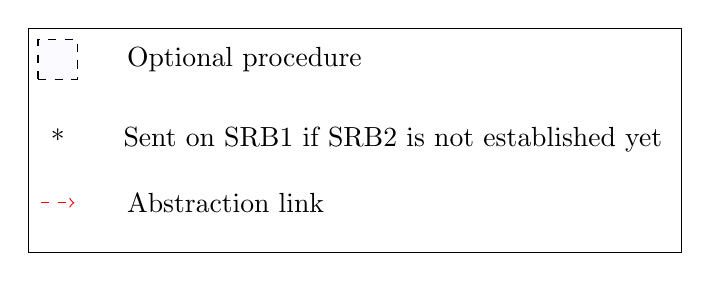
\begin{tikzpicture}
  \node[backgroundopt,
  minimum width=5mm,minimum height=5mm,anchor=east](l1) at (0,1){};
  \node[right=0.5cm of l1.center](ct1) at (0,1){Optional procedure};
  \node[below=0.5cm of l1](l2) {*};
  \node[right=0.5cm of l2](ct2) {Sent on SRB1 if SRB2 is not established yet};
  \draw[minimum width=5mm,minimum height=5mm,below=0.3cm of l2,->,dashed, draw=red]
  ($(l2.south west) - (0,0.55cm)$) -- node(l3){} ($(l2.south east) - (0,0.55cm)$);
  \node[right=0.5cm of l3.north east](ct3) {Abstraction link};
  \node[draw,fit=(ct1)(l1)(ct2)(l2)(ct3)(l3)] {};
%   \node[below = 0.5cm of l2](l3) {};
%   \draw[below=0.5cm of l2, ->] (1,1) -- (0,1);
  \end{tikzpicture}
\end{figure}
\end{center}

\begin{landscape}
\begin{figure}
\begin{center}
  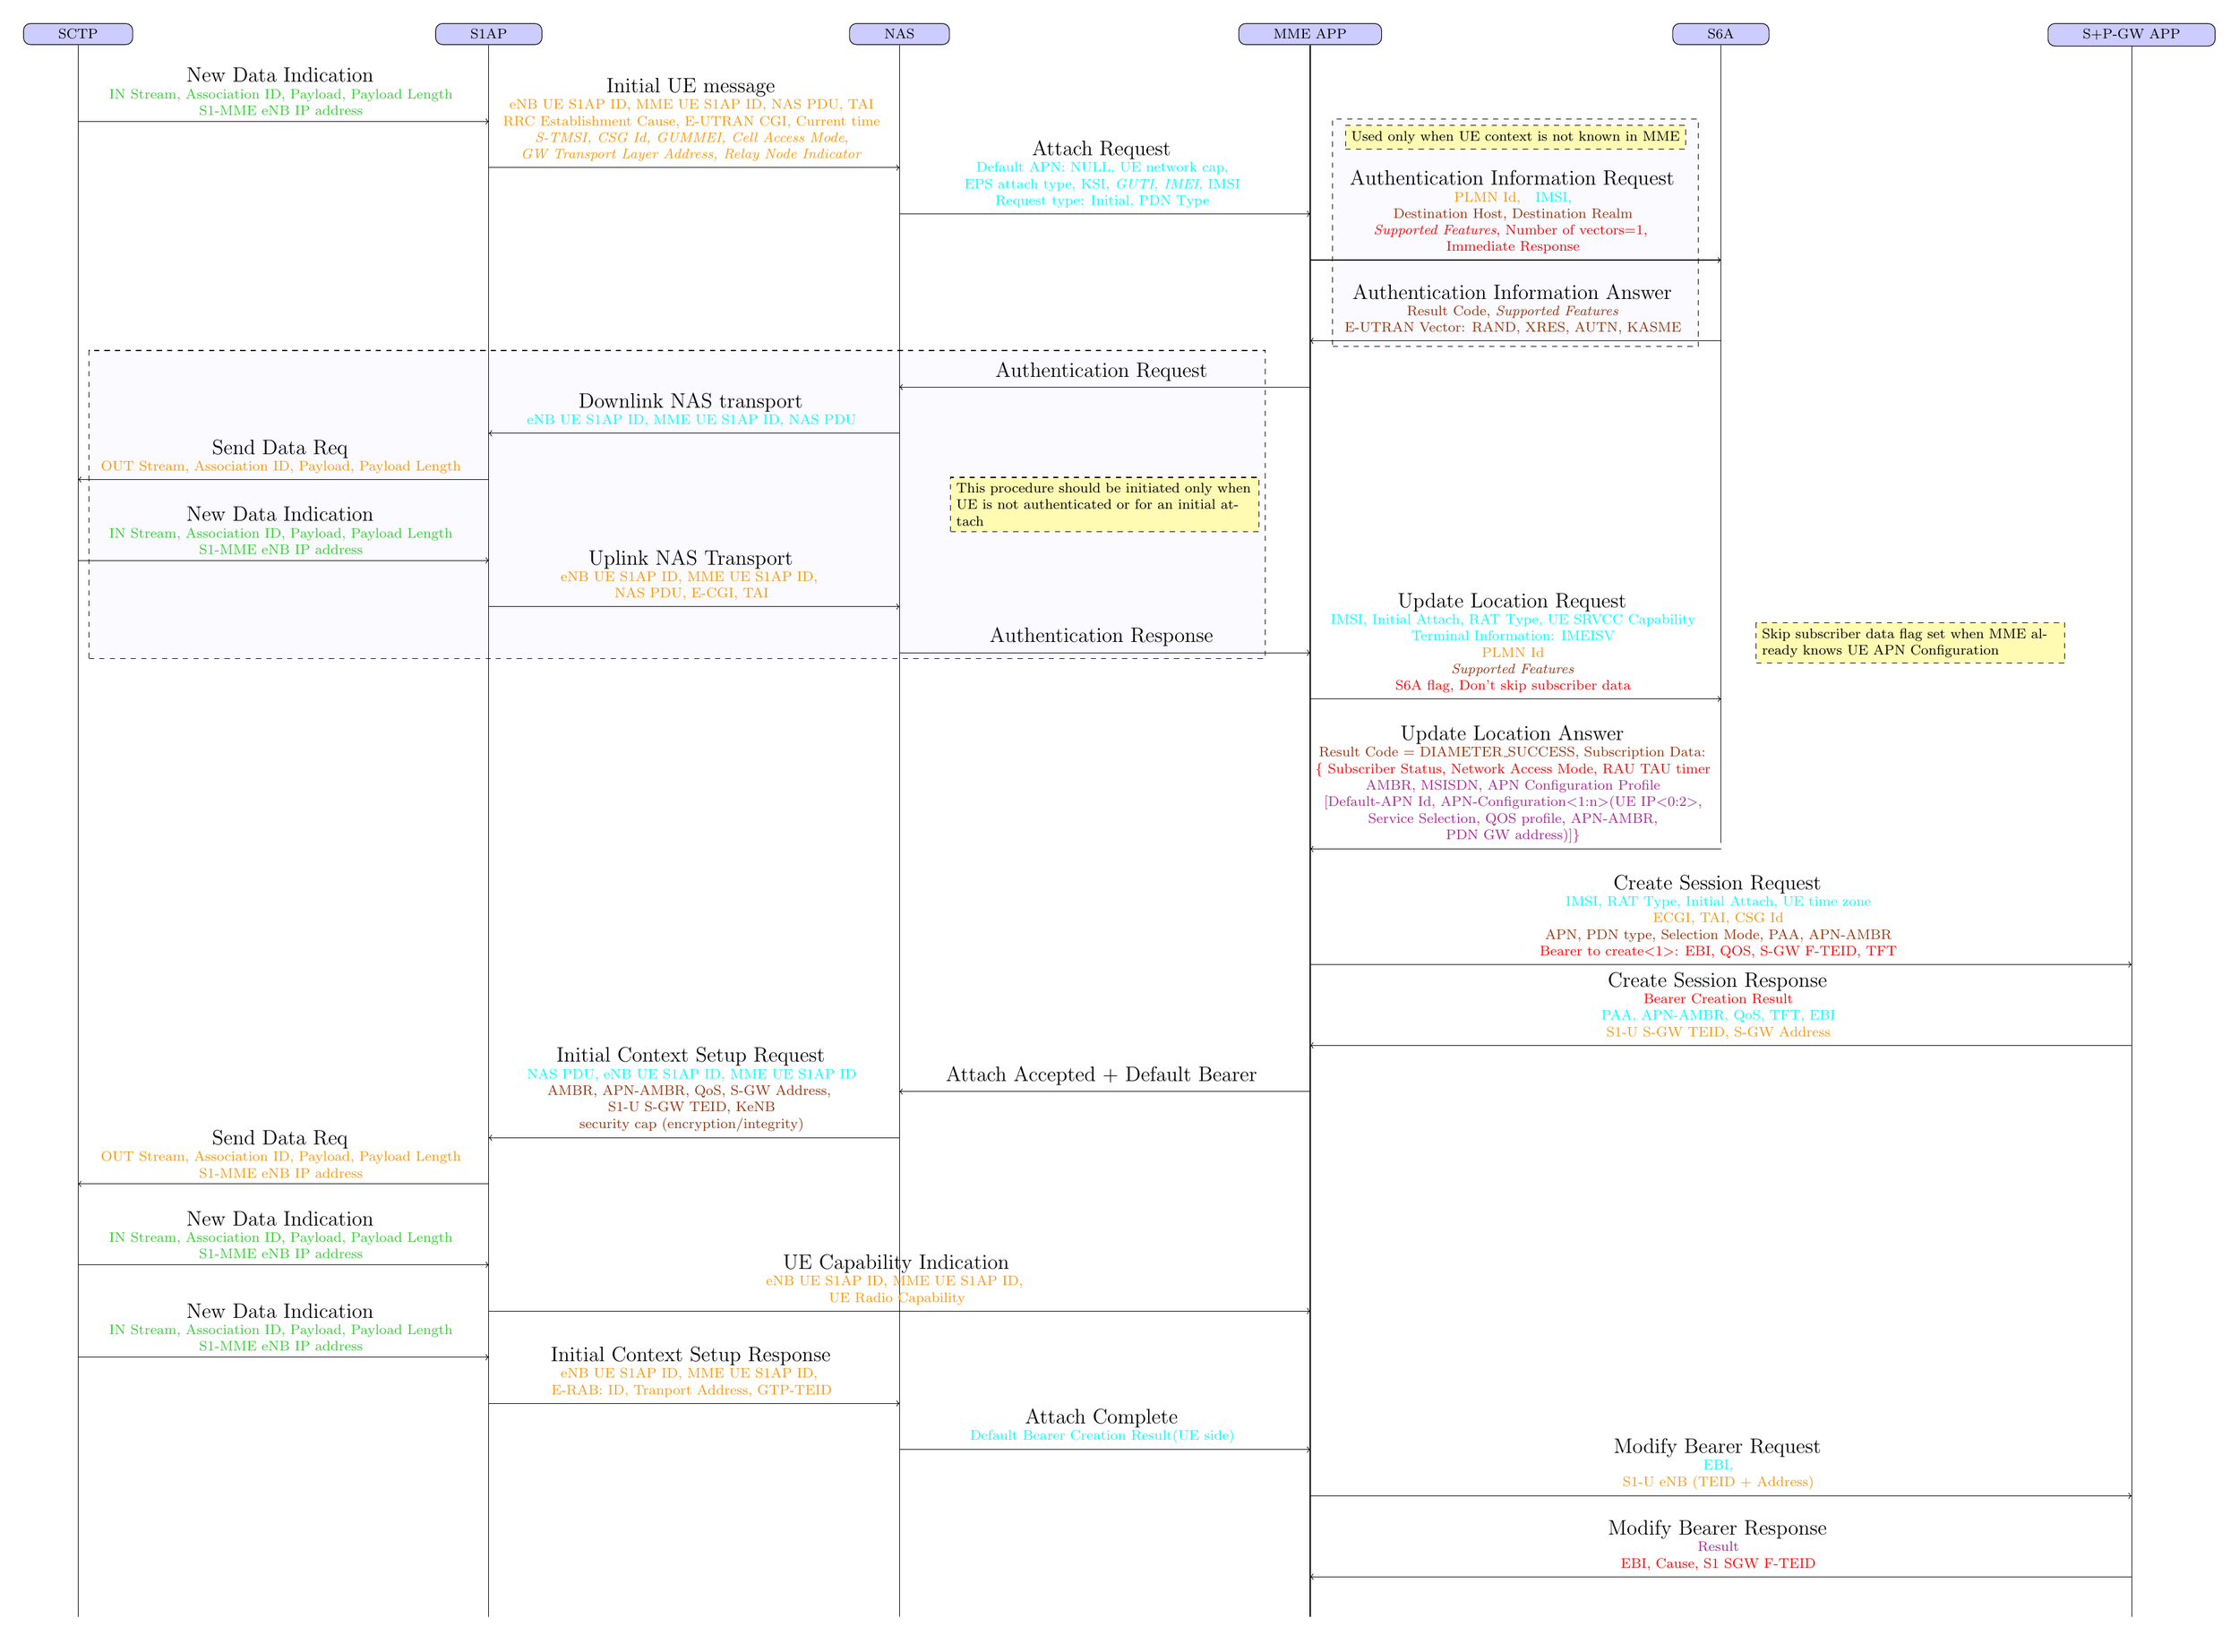
\begin{tikzpicture}[auto]
  \tikzstyle{every node}=[font=\footnotesize]
  \matrix (matrix2) [row sep=0.7cm, column sep={8.3cm,between origins}, matrix of nodes] {
      \node(SCTP) [schritt] {SCTP}; & \node(S1AP) [schritt] {S1AP};  & \node(NAS) [schritt] {NAS}; & \node(MMEAPP) [schritt] {MME APP}; & \node(S6A) [schritt] {S6A}; & \node(SPAPP) [schritt] {S+P-GW APP};\\\\
      \node(SCTP1) [] {}; & \node(S1AP1) [] {};\\
      & \node(S1AP2) [] {}; & \node(NAS1) [] {};\\
      & & \node(NAS2) [] {}; & \node(MMEAPP1) [] {};\\
      & & & \node(MMEAPP2) [] {}; & \node(S6A1) [] {};\\\\
      & & & \node(MMEAPP3) [] {}; & \node(S6A2) [] {};\\
      & & \node(NAS3) [] {}; & \node(MMEAPP4) [] {};\\
      & \node(S1AP3) [] {}; & \node(NAS4) [] {};\\
      \node(SCTP2) [] {}; & \node(S1AP4) [] {};\\\\
      \node(SCTP3) [] {}; & \node(S1AP5) [] {};\\
      & \node(S1AP6) [] {}; & \node(NAS5) [] {};\\
      & & \node(NAS6) [] {}; & \node(MMEAPP5) [] {};\\
      & & & \node(MMEAPP6) [] {}; & \node(S6A3) [] {};\\\\\\\\
      & & & \node(MMEAPP7) [] {}; & \node(S6A4) [] {};\\\\\\
      & & & \node(MMEAPP8) [] {}; & & \node(SPAPP1) [] {};\\\\
      & & & \node(MMEAPP9) [] {}; & & \node(SPAPP2) [] {};\\
      & & \node(NAS7) [] {}; & \node(MMEAPP10) [] {};\\
      & \node(S1AP7) [] {}; & \node(NAS8) [] {};\\
      \node(SCTP4) [] {}; & \node(S1AP8) [] {};\\\\
      \node(SCTP5) [] {}; & \node(S1AP9) [] {};\\
      & \node(S1AP10) [] {}; & & \node(MMEAPP11) [] {};\\
      \node(SCTP6) [] {}; & \node(S1AP11) [] {};\\
      & \node(S1AP12) [] {}; & \node(NAS9) [] {};\\
      & & \node(NAS10) [] {}; & \node(MMEAPP12) [] {};\\
      & & & \node(MMEAPP13) [] {}; & & \node(SPAPP3) [] {};\\\\
      & & & \node(MMEAPP14) [] {}; & & \node(SPAPP4) [] {};\\
      \node(SCTPEND) [] {}; & \node(S1APEND) [] {}; & \node(NASEND) [] {}; & \node(MMEAPPEND) [] {}; & \node(S6AEND) [] {}; & \node(SPAPPEND) [] {};\\
  };

  \path[-]
  (SCTP)   edge (SCTPEND)
  (S1AP)   edge (S1APEND)
  (NAS)    edge (NASEND)
  (MMEAPP) edge (MMEAPPEND)
  (S6A)    edge (S6A4)
  (SPAPP)  edge (SPAPPEND)
  ;

  \draw[->] (node cs:name=SCTP1,anchor=center) -- node(arrow1)[above, align=center]{
      \commandname{New Data Indication}
      \\\sctpcolor{IN Stream, Association ID, Payload, Payload Length}
      \\\sctpcolor{S1-MME eNB IP address}}(node cs:name=S1AP1,anchor=center);
  \draw[->] (node cs:name=S1AP2,anchor=center) -- node(arrow2)[above, align=center]{
      \commandname{Initial UE message}
      \\\soneapcolor{eNB UE S1AP ID, MME UE S1AP ID, NAS PDU, TAI}
      \\\soneapcolor{RRC Establishment Cause, E-UTRAN CGI, Current time}
      \\\soneapcolor{\emph{S-TMSI, CSG Id, GUMMEI, Cell Access Mode},}
      \\\soneapcolor{\emph{GW Transport Layer Address, Relay Node Indicator}}}(node cs:name=NAS1,anchor=center);
  \draw[->] (node cs:name=NAS2,anchor=center) -- node(arrow3)[above, align=center]{
      \commandname{Attach Request}
      \\\nascolor{Default APN: NULL, UE network cap,}
      \\\nascolor{EPS attach type, KSI, \emph{GUTI, IMEI}, IMSI}
      \\\nascolor{Request type: Initial, PDN Type}}(node cs:name=MMEAPP1,anchor=center);
  \draw[->] (node cs:name=MMEAPP2,anchor=center) -- node(arrow4)[above, align=center]{
      \commandname{Authentication Information Request}
      \\\soneapcolor{PLMN Id, }\nascolor{IMSI,}
      \\\ssixcolor{Destination Host, Destination Realm}
      \\\mmecolor{\emph{Supported Features}, Number of vectors=1, }
      \\\mmecolor{Immediate Response}}(node cs:name=S6A1,anchor=center);
  \draw[->] (node cs:name=S6A2,anchor=center) -- node(arrow5)[above, align=center]{
      \commandname{Authentication Information Answer}
      \\\ssixcolor{Result Code, \emph{Supported Features}}
      \\\ssixcolor{E-UTRAN Vector: RAND, XRES, AUTN, KASME}}(node cs:name=MMEAPP3,anchor=center);
  \draw[->] (node cs:name=MMEAPP4,anchor=center) -- node(arrow6)[above, align=center]{
      \commandname{Authentication Request}}(node cs:name=NAS3,anchor=center);
  \draw[->] (node cs:name=NAS4,anchor=center) -- node(arrow7)[above, align=center]{
      \commandname{Downlink NAS transport}
      \\\nascolor{eNB UE S1AP ID, MME UE S1AP ID, NAS PDU}}(node cs:name=S1AP3,anchor=center);
  \draw[->] (node cs:name=S1AP4,anchor=center) -- node(arrow8)[above, align=center]{
      \commandname{Send Data Req}
      \\\soneapcolor{OUT Stream, Association ID, Payload, Payload Length}}(node cs:name=SCTP2,anchor=center);
  \draw[->] (node cs:name=SCTP3,anchor=center) -- node(arrow9)[above, align=center]{
      \commandname{New Data Indication}
      \\\sctpcolor{IN Stream, Association ID, Payload, Payload Length}
      \\\sctpcolor{S1-MME eNB IP address}}(node cs:name=S1AP5,anchor=center);
  \draw[->] (node cs:name=S1AP6,anchor=center) -- node(arrow10)[above, align=center]{
      \commandname{Uplink NAS Transport}
      \\\soneapcolor{eNB UE S1AP ID, MME UE S1AP ID, }
      \\\soneapcolor{NAS PDU, E-CGI, TAI}}(node cs:name=NAS5,anchor=center);
  \draw[->] (node cs:name=NAS6,anchor=center) -- node(arrow11)[above, align=center]{
      \commandname{Authentication Response}}(node cs:name=MMEAPP5,anchor=center);
  \draw[->] (node cs:name=MMEAPP6,anchor=center) -- node(arrow12)[above, align=center]{
      \commandname{Update Location Request}
      \\\nascolor{IMSI, Initial Attach, RAT Type, UE SRVCC Capability}
      \\\nascolor{Terminal Information: IMEISV}
      \\\soneapcolor{PLMN Id}
      \\\ssixcolor{\emph{Supported Features}}
      \\\mmecolor{S6A flag, Don't skip subscriber data}}(node cs:name=S6A3,anchor=center);
  \draw[->] (node cs:name=S6A4,anchor=center) -- node(arrow13)[above, align=center]{
      \commandname{Update Location Answer}
      \\\ssixcolor{Result Code = DIAMETER\_SUCCESS, Subscription Data:}
      \\\mmecolor{\{ Subscriber Status, Network Access Mode, RAU TAU timer}
      \\\spappcolor{AMBR, MSISDN, APN Configuration Profile}
      \\\spappcolor{[Default-APN Id, APN-Configuration$<$1:n$>$(UE IP$<$0:2$>$,}
      \\\spappcolor{Service Selection, QOS profile, APN-AMBR,}
      \\\spappcolor{PDN GW address)]\}}}(node cs:name=MMEAPP7,anchor=center);
  \draw[->] (node cs:name=MMEAPP8,anchor=center) -- node(arrow14)[above, align=center]{
      \commandname{Create Session Request}
      \\\nascolor{IMSI, RAT Type, Initial Attach, UE time zone}
      \\\soneapcolor{ECGI, TAI, CSG Id}
      \\\ssixcolor{APN, PDN type, Selection Mode, PAA, APN-AMBR}
      \\\mmecolor{Bearer to create$<$1$>$: EBI, QOS, S-GW F-TEID, TFT}}(node cs:name=SPAPP1,anchor=center);
  \draw[->] (node cs:name=SPAPP2,anchor=center) -- node(arrow15)[above, align=center]{
      \commandname{Create Session Response}
      \\\mmecolor{Bearer Creation Result}
      \\\nascolor{PAA, APN-AMBR, QoS, TFT, EBI}
      \\\soneapcolor{S1-U S-GW TEID, S-GW Address}}(node cs:name=MMEAPP9,anchor=center);
  \draw[->] (node cs:name=MMEAPP10,anchor=center) -- node(arrow16)[above, align=center]{
      \commandname{Attach Accepted + Default Bearer}}(node cs:name=NAS7,anchor=center);
  \draw[->] (node cs:name=NAS8,anchor=center) -- node(arrow17)[above, align=center]{
      \commandname{Initial Context Setup Request}
      \\\nascolor{NAS PDU, eNB UE S1AP ID, MME UE S1AP ID}
      \\\ssixcolor{AMBR, APN-AMBR, QoS, S-GW Address, }
      \\\ssixcolor{S1-U S-GW TEID, KeNB}
      \\\ssixcolor{security cap (encryption/integrity)}}(node cs:name=S1AP7,anchor=center);
  \draw[->] (node cs:name=S1AP8,anchor=center) -- node(arrow18)[above, align=center]{
      \commandname{Send Data Req}
      \\\soneapcolor{OUT Stream, Association ID, Payload, Payload Length}
      \\\soneapcolor{S1-MME eNB IP address}}(node cs:name=SCTP4,anchor=center);
  \draw[->] (node cs:name=SCTP5,anchor=center) -- node(arrow19)[above, align=center]{
      \commandname{New Data Indication}
      \\\sctpcolor{IN Stream, Association ID, Payload, Payload Length}
      \\\sctpcolor{S1-MME eNB IP address}}(node cs:name=S1AP9,anchor=center);
  \draw[->] (node cs:name=S1AP10,anchor=center) -- node(arrow20)[above, align=center]{
      \commandname{UE Capability Indication}
      \\\soneapcolor{eNB UE S1AP ID, MME UE S1AP ID, }
      \\\soneapcolor{UE Radio Capability}}(node cs:name=MMEAPP11,anchor=center);
  \draw[->] (node cs:name=SCTP6,anchor=center) -- node(arrow21)[above, align=center]{
      \commandname{New Data Indication}
      \\\sctpcolor{IN Stream, Association ID, Payload, Payload Length}
      \\\sctpcolor{S1-MME eNB IP address}}(node cs:name=S1AP11,anchor=center);
  \draw[->] (node cs:name=S1AP12,anchor=center) -- node(arrow22)[above, align=center]{
      \commandname{Initial Context Setup Response}
      \\\soneapcolor{eNB UE S1AP ID, MME UE S1AP ID, }
      \\\soneapcolor{E-RAB: ID, Tranport Address, GTP-TEID}}(node cs:name=NAS9,anchor=center);
  \draw[->] (node cs:name=NAS10,anchor=center) -- node(arrow23)[above, align=center]{
      \commandname{Attach Complete}
      \\\nascolor{Default Bearer Creation Result(UE side)}}(node cs:name=MMEAPP12,anchor=center);
  \draw[->] (node cs:name=MMEAPP13,anchor=center) -- node(arrow24)[above, align=center]{
      \commandname{Modify Bearer Request}
      \\\nascolor{EBI,}
      \\\soneapcolor{S1-U eNB (TEID + Address)}}(node cs:name=SPAPP3,anchor=center);
  \draw[->] (node cs:name=SPAPP4,anchor=center) -- node(arrow25)[above, align=center]{
      \commandname{Modify Bearer Response}
      \\\spappcolor{Result}
      \\\mmecolor{EBI, Cause, S1 SGW F-TEID}}(node cs:name=MMEAPP14,anchor=center);

  \node[above=3mm of arrow4, backgroundcomment] (opt1) {Used only when UE context is not known in MME};
  \begin{pgfonlayer}{background}
  \node[fit=(arrow4)(arrow5)(opt1), backgroundopt] {};
  \end{pgfonlayer}
  \node[right=of arrow12, backgroundcomment, text width=6cm] {Skip subscriber data flag set when MME already knows UE APN Configuration};

  \node(opt2) at ($(arrow6)!0.5!(arrow11)$) [backgroundcomment, text width=6cm] {This procedure should be initiated only when UE is not authenticated or for an initial attach};
  \begin{pgfonlayer}{background}
  \node[fit=(arrow6)(arrow9)(arrow8)(arrow11)(opt2), backgroundopt] {};
  \end{pgfonlayer}

  \end{tikzpicture}
  \end{center}
  \caption{MME detailed behaviour: Default Bearer Creation} \label{fig:MME detailed behaviour}
  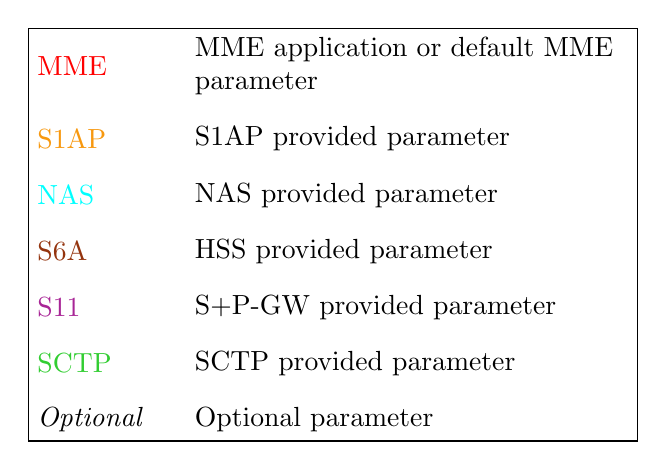
\begin{tikzpicture}
  \matrix (matrix3) [square matrix] {
      \node[](l1) {\mmecolor{MME}};         & \node[](ct1) {MME application or default MME parameter};\\
      \node[](l2) {\soneapcolor{S1AP}};     & \node[](ct2) {S1AP provided parameter};\\
      \node[](l3) {\nascolor{NAS}};         & \node[](ct3) {NAS provided parameter};\\
      \node[](l4) {\ssixcolor{S6A}};        & \node[](ct4) {HSS provided parameter};\\
      \node[](l5) {\spappcolor{S11}};       & \node[](ct5) {S+P-GW provided parameter};\\
      \node[](l6) {\sctpcolor{SCTP}};       & \node[](ct6) {SCTP provided parameter};\\
      \node[](l7) {\emph{Optional}};        & \node[](ct7) {Optional parameter};\\
  };

%   \node[draw,fit=(ct1)(l1)(ct2)(l2)(ct3)(l3)(l4)(ct4)(l5)(ct5)] {};
  %   \node[below = 0.5cm of l2](l3) {};
  %   \draw[below=0.5cm of l2, ->] (1,1) -- (0,1);
  \end{tikzpicture}
  \end{figure}
  \end{landscape}

  \begin{landscape}
  \begin{figure}
  \begin{center}
  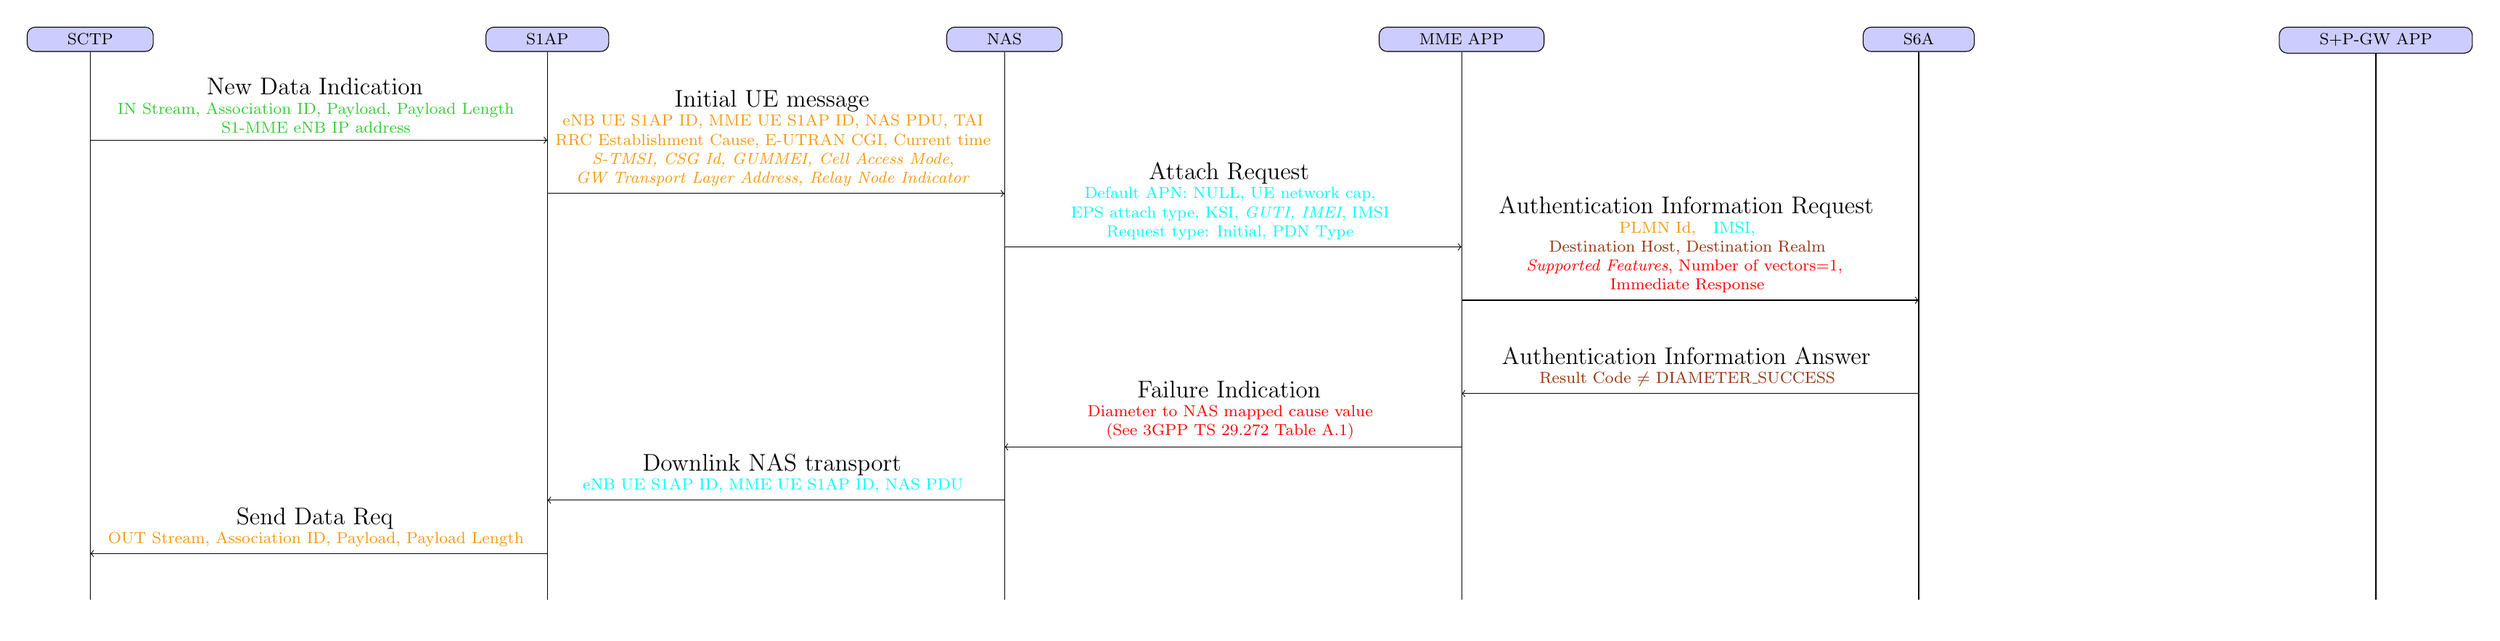
\begin{tikzpicture}
  \tikzstyle{every node}=[font=\footnotesize]
  \matrix (matrix3) [row sep=0.7cm, column sep={8cm,between origins}, matrix of nodes] {
      \node(SCTP) [schritt] {SCTP}; & \node(S1AP) [schritt] {S1AP};  & \node(NAS) [schritt] {NAS}; & \node(MMEAPP) [schritt] {MME APP}; & \node(S6A) [schritt] {S6A}; & \node(SPAPP) [schritt] {S+P-GW APP};\\\\
      \node(SCTP1) [] {}; & \node(S1AP1) [] {};\\
      & \node(S1AP2) [] {}; & \node(NAS1) [] {};\\
      & & \node(NAS2) [] {}; & \node(MMEAPP1) [] {};\\
      & & & \node(MMEAPP2) [] {}; & \node(S6A1) [] {};\\\\
      & & & \node(MMEAPP3) [] {}; & \node(S6A2) [] {};\\
      & & \node(NAS3) [] {}; & \node(MMEAPP4) [] {};\\
      & \node(S1AP3) [] {}; & \node(NAS4) [] {};\\
      \node(SCTP2) [] {}; & \node(S1AP4) [] {};\\
      \node(SCTPEND) [] {}; & \node(S1APEND) [] {}; & \node(NASEND) [] {}; & \node(MMEAPPEND) [] {}; & \node(S6AEND) [] {}; & \node(SPAPPEND) [] {};\\
  };

  \path[-]
  (SCTP)   edge (SCTPEND)
  (S1AP)   edge (S1APEND)
  (NAS)    edge (NASEND)
  (MMEAPP) edge (MMEAPPEND)
  (S6A)    edge (S6AEND)
  (SPAPP)  edge (SPAPPEND)
  ;

  \draw[->] (node cs:name=SCTP1,anchor=center) -- node(arrow1)[above, align=center]{
      \commandname{New Data Indication}
      \\\sctpcolor{IN Stream, Association ID, Payload, Payload Length}
      \\\sctpcolor{S1-MME eNB IP address}}(node cs:name=S1AP1,anchor=center);
  \draw[->] (node cs:name=S1AP2,anchor=center) -- node(arrow2)[above, align=center]{
      \commandname{Initial UE message}
      \\\soneapcolor{eNB UE S1AP ID, MME UE S1AP ID, NAS PDU, TAI}
      \\\soneapcolor{RRC Establishment Cause, E-UTRAN CGI, Current time}
      \\\soneapcolor{\emph{S-TMSI, CSG Id, GUMMEI, Cell Access Mode},}
      \\\soneapcolor{\emph{GW Transport Layer Address, Relay Node Indicator}}}(node cs:name=NAS1,anchor=center);
  \draw[->] (node cs:name=NAS2,anchor=center) -- node(arrow3)[above, align=center]{
      \commandname{Attach Request}
      \\\nascolor{Default APN: NULL, UE network cap,}
      \\\nascolor{EPS attach type, KSI, \emph{GUTI, IMEI}, IMSI}
      \\\nascolor{Request type: Initial, PDN Type}}(node cs:name=MMEAPP1,anchor=center);
  \draw[->] (node cs:name=MMEAPP2,anchor=center) -- node(arrow4)[above, align=center]{
      \commandname{Authentication Information Request}
      \\\soneapcolor{PLMN Id, }\nascolor{IMSI,}
      \\\ssixcolor{Destination Host, Destination Realm}
      \\\mmecolor{\emph{Supported Features}, Number of vectors=1, }
      \\\mmecolor{Immediate Response}}(node cs:name=S6A1,anchor=center);
  \draw[->] (node cs:name=S6A2,anchor=center) -- node(arrow5)[above, align=center]{
      \commandname{Authentication Information Answer}
      \\\ssixcolor{Result Code $\neq$ DIAMETER\_SUCCESS}}
    (node cs:name=MMEAPP3,anchor=center);
  \draw[->] (node cs:name=MMEAPP4,anchor=center) -- node(arrow6)[above, align=center]{
      \commandname{Failure Indication}
      \\\mmecolor{Diameter to NAS mapped cause value}
      \\\mmecolor{(See 3GPP TS 29.272 Table A.1)}}
    (node cs:name=NAS3,anchor=center);
  \draw[->] (node cs:name=NAS4,anchor=center) -- node(arrow7)[above, align=center]{
      \commandname{Downlink NAS transport}
      \\\nascolor{eNB UE S1AP ID, MME UE S1AP ID, NAS PDU}}
    (node cs:name=S1AP3,anchor=center);
  \draw[->] (node cs:name=S1AP4,anchor=center) -- node(arrow8)[above, align=center]{
      \commandname{Send Data Req}
      \\\soneapcolor{OUT Stream, Association ID, Payload, Payload Length}}
    (node cs:name=SCTP2,anchor=center);
  \end{tikzpicture}
  \end{center}
  \caption{MME detailed behaviour: Default Bearer Rejected (S6A Authentication Failure)} \label{fig:MME detailed behaviour: Default Bearer Rejected (S6A Failure)}

  \begin{center}
  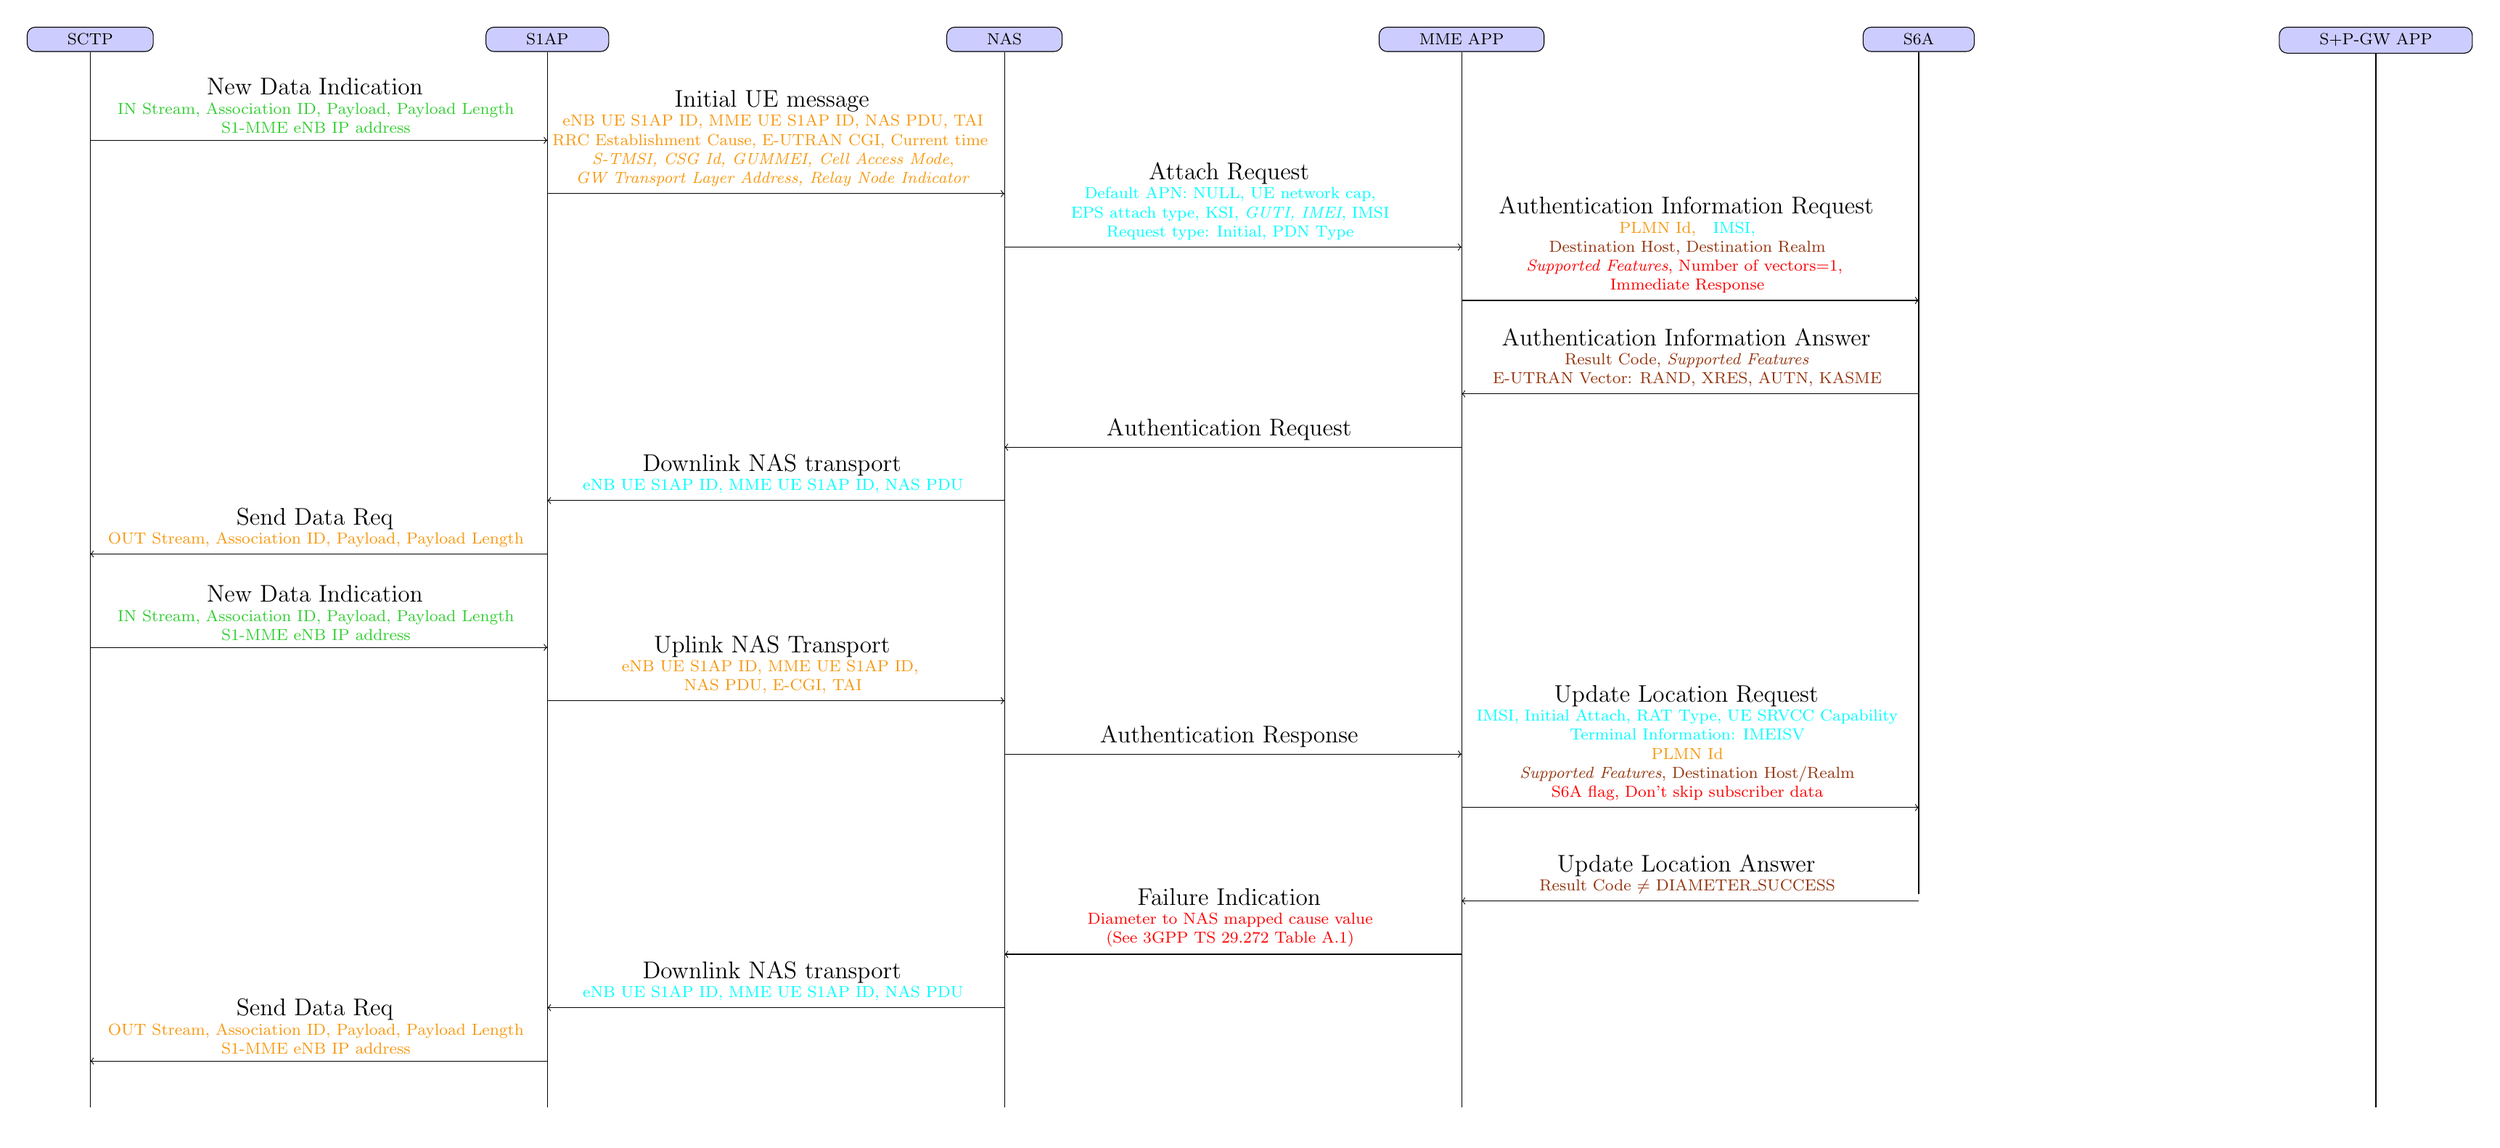
\begin{tikzpicture}
  \tikzstyle{every node}=[font=\footnotesize]
  \matrix (matrix4) [row sep=0.7cm, column sep={8cm,between origins}, matrix of nodes] {
      \node(SCTP) [schritt] {SCTP}; & \node(S1AP) [schritt] {S1AP};  & \node(NAS) [schritt] {NAS}; & \node(MMEAPP) [schritt] {MME APP}; & \node(S6A) [schritt] {S6A}; & \node(SPAPP) [schritt] {S+P-GW APP};\\\\
      \node(SCTP1) [] {}; & \node(S1AP1) [] {};\\
      & \node(S1AP2) [] {}; & \node(NAS1) [] {};\\
      & & \node(NAS2) [] {}; & \node(MMEAPP1) [] {};\\
      & & & \node(MMEAPP2) [] {}; & \node(S6A1) [] {};\\\\
      & & & \node(MMEAPP3) [] {}; & \node(S6A2) [] {};\\
      & & \node(NAS3) [] {}; & \node(MMEAPP4) [] {};\\
      & \node(S1AP3) [] {}; & \node(NAS4) [] {};\\
      \node(SCTP2) [] {}; & \node(S1AP4) [] {};\\\\
      \node(SCTP3) [] {}; & \node(S1AP5) [] {};\\
      & \node(S1AP6) [] {}; & \node(NAS5) [] {};\\
      & & \node(NAS6) [] {}; & \node(MMEAPP5) [] {};\\
      & & & \node(MMEAPP6) [] {}; & \node(S6A3) [] {};\\\\
      & & & \node(MMEAPP7) [] {}; & \node(S6A4) [] {};\\
      & & \node(NAS7) [] {}; & \node(MMEAPP10) [] {};\\
      & \node(S1AP7) [] {}; & \node(NAS8) [] {};\\
      \node(SCTP4) [] {}; & \node(S1AP8) [] {};\\
      \node(SCTPEND) [] {}; & \node(S1APEND) [] {}; & \node(NASEND) [] {}; & \node(MMEAPPEND) [] {}; & \node(S6AEND) [] {}; & \node(SPAPPEND) [] {};\\
  };

  \path[-]
  (SCTP)   edge (SCTPEND)
  (S1AP)   edge (S1APEND)
  (NAS)    edge (NASEND)
  (MMEAPP) edge (MMEAPPEND)
  (S6A)    edge (S6A4)
  (SPAPP)  edge (SPAPPEND)
  ;

  \draw[->] (node cs:name=SCTP1,anchor=center) -- node(arrow1)[above, align=center]{
      \commandname{New Data Indication}
      \\\sctpcolor{IN Stream, Association ID, Payload, Payload Length}
      \\\sctpcolor{S1-MME eNB IP address}}(node cs:name=S1AP1,anchor=center);
  \draw[->] (node cs:name=S1AP2,anchor=center) -- node(arrow2)[above, align=center]{
      \commandname{Initial UE message}
      \\\soneapcolor{eNB UE S1AP ID, MME UE S1AP ID, NAS PDU, TAI}
      \\\soneapcolor{RRC Establishment Cause, E-UTRAN CGI, Current time }
      \\\soneapcolor{\emph{S-TMSI, CSG Id, GUMMEI, Cell Access Mode},}
      \\\soneapcolor{\emph{GW Transport Layer Address, Relay Node Indicator}}}(node cs:name=NAS1,anchor=center);
  \draw[->] (node cs:name=NAS2,anchor=center) -- node(arrow3)[above, align=center]{
      \commandname{Attach Request}
      \\\nascolor{Default APN: NULL, UE network cap,}
      \\\nascolor{EPS attach type, KSI, \emph{GUTI, IMEI}, IMSI}
      \\\nascolor{Request type: Initial, PDN Type}}(node cs:name=MMEAPP1,anchor=center);
  \draw[->] (node cs:name=MMEAPP2,anchor=center) -- node(arrow4)[above, align=center]{
      \commandname{Authentication Information Request}
      \\\soneapcolor{PLMN Id, }\nascolor{IMSI,}
      \\\ssixcolor{Destination Host, Destination Realm}
      \\\mmecolor{\emph{Supported Features}, Number of vectors=1, }
      \\\mmecolor{Immediate Response}}(node cs:name=S6A1,anchor=center);
  \draw[->] (node cs:name=S6A2,anchor=center) -- node(arrow5)[above, align=center]{
      \commandname{Authentication Information Answer}
      \\\ssixcolor{Result Code, \emph{Supported Features}}
      \\\ssixcolor{E-UTRAN Vector: RAND, XRES, AUTN, KASME}}(node cs:name=MMEAPP3,anchor=center);
  \draw[->] (node cs:name=MMEAPP4,anchor=center) -- node(arrow6)[above, align=center]{
      \commandname{Authentication Request}}(node cs:name=NAS3,anchor=center);
  \draw[->] (node cs:name=NAS4,anchor=center) -- node(arrow7)[above, align=center]{
      \commandname{Downlink NAS transport}
      \\\nascolor{eNB UE S1AP ID, MME UE S1AP ID, NAS PDU}}(node cs:name=S1AP3,anchor=center);
  \draw[->] (node cs:name=S1AP4,anchor=center) -- node(arrow8)[above, align=center]{
      \commandname{Send Data Req}
      \\\soneapcolor{OUT Stream, Association ID, Payload, Payload Length}}(node cs:name=SCTP2,anchor=center);
  \draw[->] (node cs:name=SCTP3,anchor=center) -- node(arrow9)[above, align=center]{
      \commandname{New Data Indication}
      \\\sctpcolor{IN Stream, Association ID, Payload, Payload Length}
      \\\sctpcolor{S1-MME eNB IP address}}(node cs:name=S1AP5,anchor=center);
  \draw[->] (node cs:name=S1AP6,anchor=center) -- node(arrow10)[above, align=center]{
      \commandname{Uplink NAS Transport}
      \\\soneapcolor{eNB UE S1AP ID, MME UE S1AP ID, }
      \\\soneapcolor{NAS PDU, E-CGI, TAI}}(node cs:name=NAS5,anchor=center);
  \draw[->] (node cs:name=NAS6,anchor=center) -- node(arrow11)[above, align=center]{
      \commandname{Authentication Response}}(node cs:name=MMEAPP5,anchor=center);
  \draw[->] (node cs:name=MMEAPP6,anchor=center) -- node(arrow12)[above, align=center]{
      \commandname{Update Location Request}
      \\\nascolor{IMSI, Initial Attach, RAT Type, UE SRVCC Capability}
      \\\nascolor{Terminal Information: IMEISV}
      \\\soneapcolor{PLMN Id}
      \\\ssixcolor{\emph{Supported Features}, Destination Host/Realm}
      \\\mmecolor{S6A flag, Don't skip subscriber data}}(node cs:name=S6A3,anchor=center);
  \draw[->] (node cs:name=S6A4,anchor=center) -- node(arrow13)[above, align=center]{
      \commandname{Update Location Answer}
      \\\ssixcolor{Result Code $\neq$ DIAMETER\_SUCCESS}}(node cs:name=MMEAPP7,anchor=center);
  \draw[->] (node cs:name=MMEAPP10,anchor=center) -- node(arrow16)[above, align=center]{
      \commandname{Failure Indication}
      \\\mmecolor{Diameter to NAS mapped cause value}
      \\\mmecolor{(See 3GPP TS 29.272 Table A.1)}}(node cs:name=NAS7,anchor=center);
  \draw[->] (node cs:name=NAS8,anchor=center) -- node(arrow17)[above, align=center]{
      \commandname{Downlink NAS transport}
      \\\nascolor{eNB UE S1AP ID, MME UE S1AP ID, NAS PDU}}(node cs:name=S1AP7,anchor=center);
  \draw[->] (node cs:name=S1AP8,anchor=center) -- node(arrow18)[above, align=center]{
      \commandname{Send Data Req}
      \\\soneapcolor{OUT Stream, Association ID, Payload, Payload Length}
      \\\soneapcolor{S1-MME eNB IP address}}(node cs:name=SCTP4,anchor=center);

  \end{tikzpicture}
  \end{center}
  \caption{MME detailed behaviour: Default Bearer Rejected (S6A Update Location Failure)} \label{fig:MME detailed behaviour: Default Bearer Rejected (S6A Update Location Failure)}
  \end{figure}
\end{landscape}

\begin{landscape}
\begin{figure}
  \begin{center}
  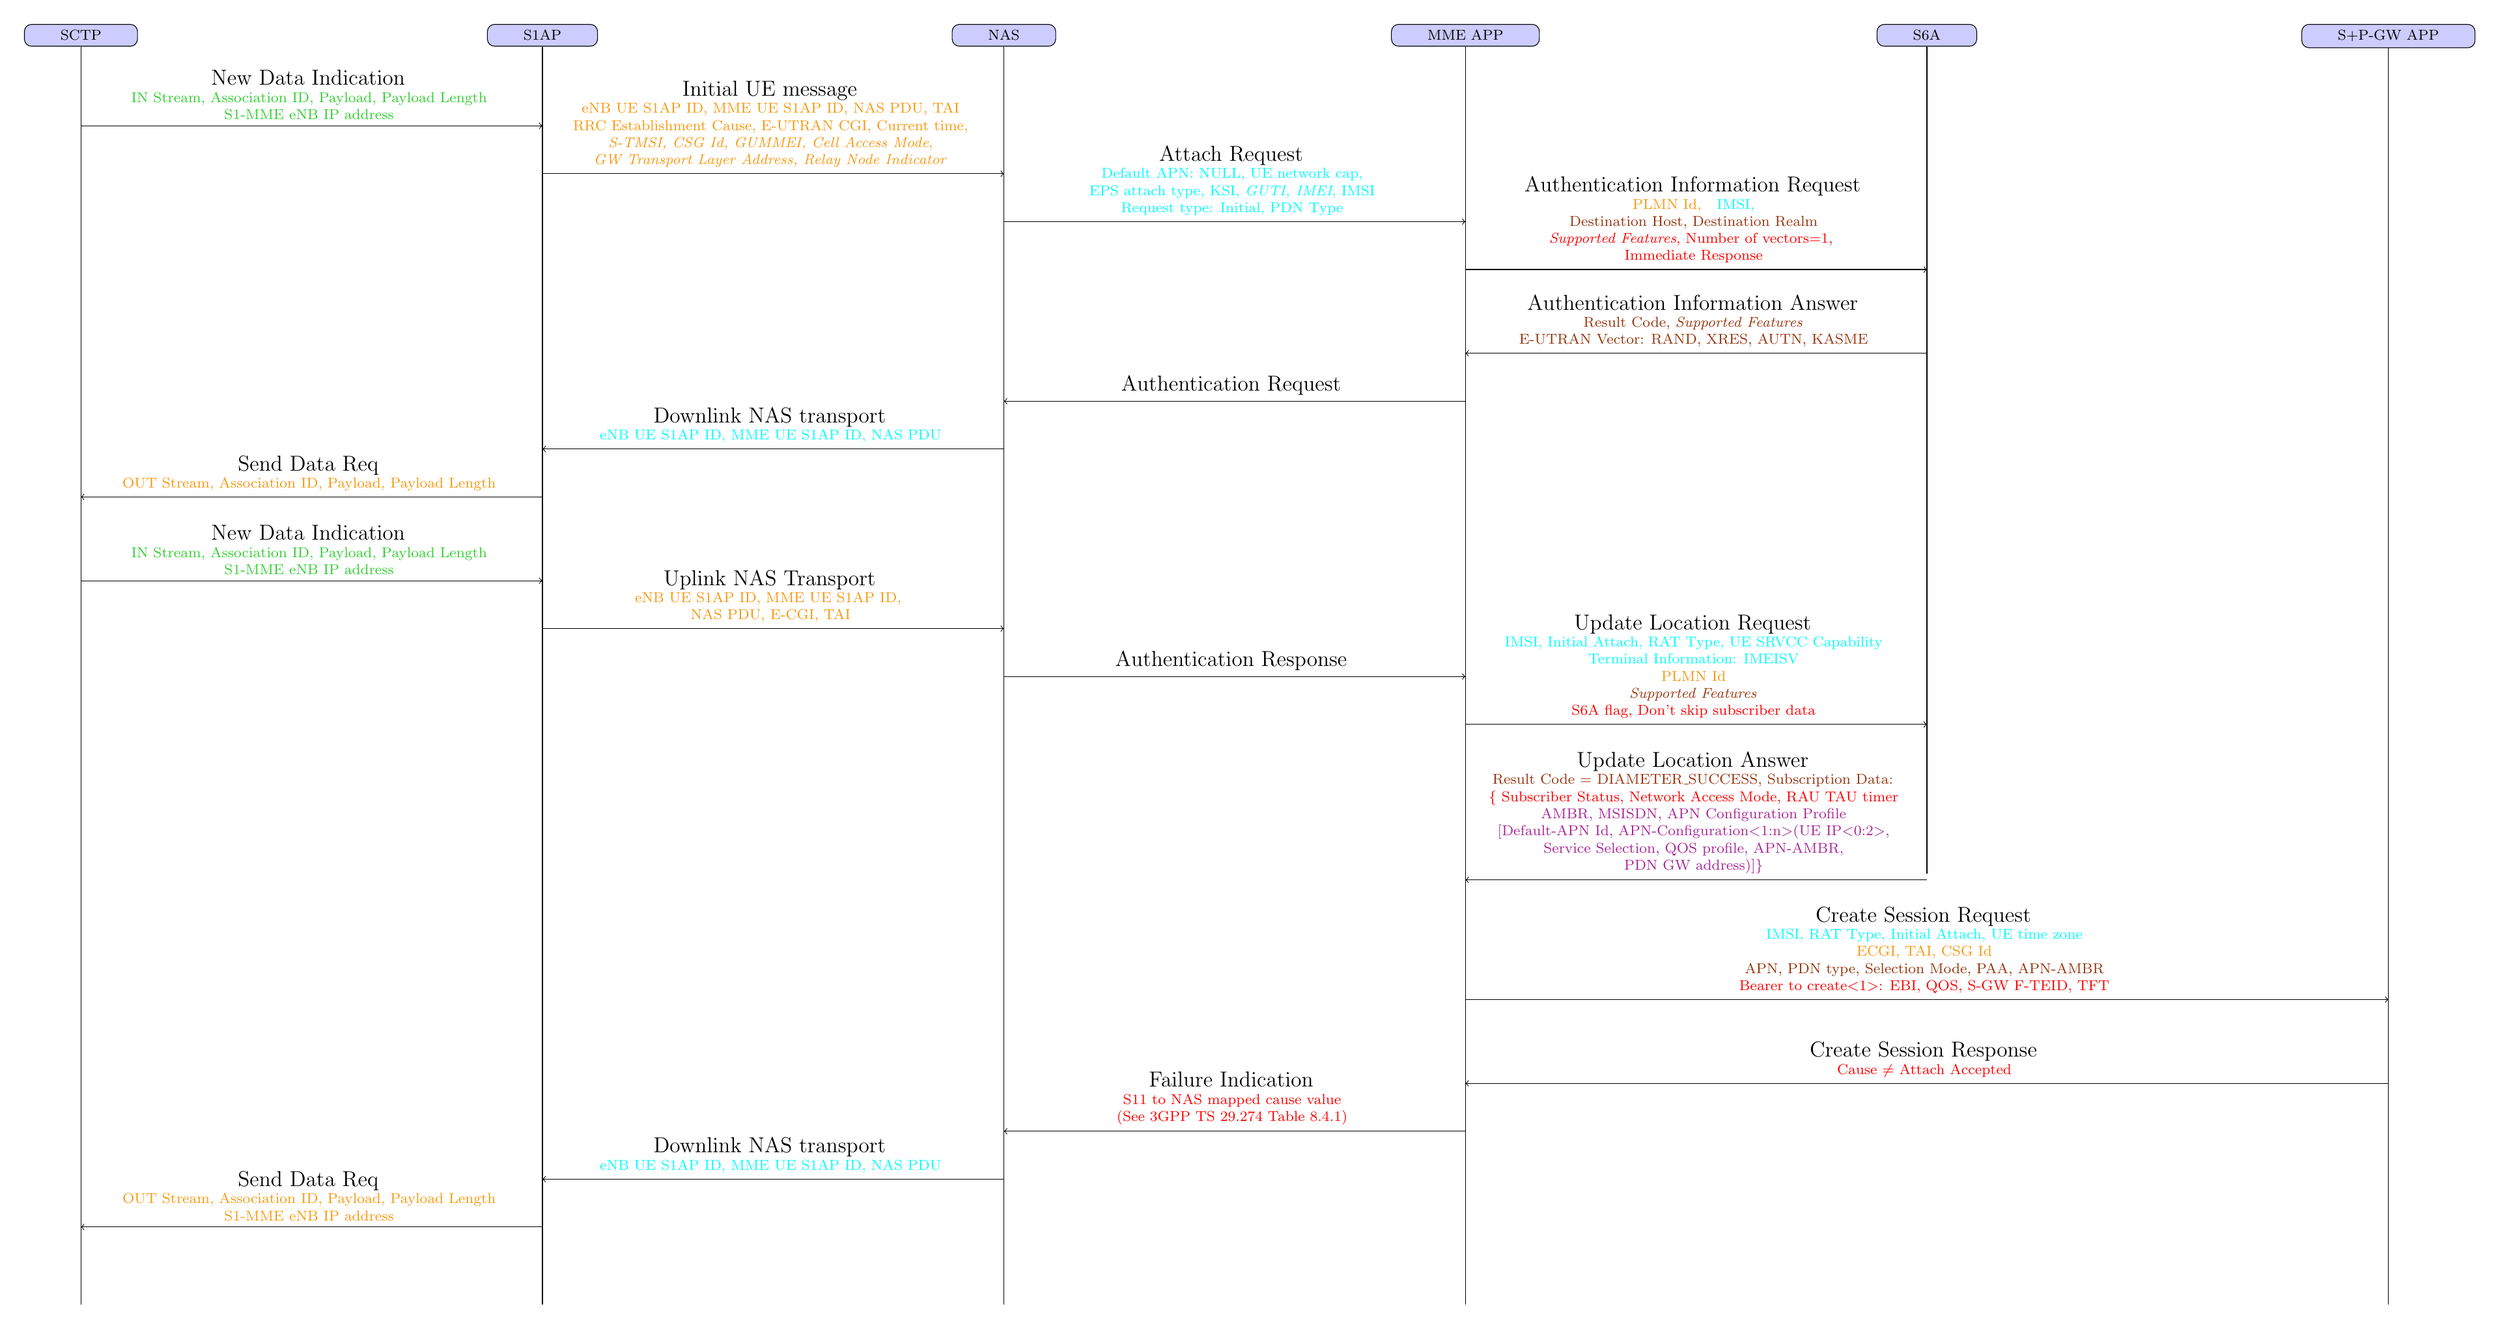
\begin{tikzpicture}
  \tikzstyle{every node}=[font=\footnotesize]
  \matrix (matrix5) [row sep=0.7cm, column sep={9cm,between origins}, matrix of nodes] {
      \node(SCTP) [schritt] {SCTP}; & \node(S1AP) [schritt] {S1AP};  & \node(NAS) [schritt] {NAS}; & \node(MMEAPP) [schritt] {MME APP}; & \node(S6A) [schritt] {S6A}; & \node(SPAPP) [schritt] {S+P-GW APP};\\\\
      \node(SCTP1) [] {}; & \node(S1AP1) [] {};\\
      & \node(S1AP2) [] {}; & \node(NAS1) [] {};\\
      & & \node(NAS2) [] {}; & \node(MMEAPP1) [] {};\\
      & & & \node(MMEAPP2) [] {}; & \node(S6A1) [] {};\\\\
      & & & \node(MMEAPP3) [] {}; & \node(S6A2) [] {};\\
      & & \node(NAS3) [] {}; & \node(MMEAPP4) [] {};\\
      & \node(S1AP3) [] {}; & \node(NAS4) [] {};\\
      \node(SCTP2) [] {}; & \node(S1AP4) [] {};\\\\
      \node(SCTP3) [] {}; & \node(S1AP5) [] {};\\
      & \node(S1AP6) [] {}; & \node(NAS5) [] {};\\
      & & \node(NAS6) [] {}; & \node(MMEAPP5) [] {};\\
      & & & \node(MMEAPP6) [] {}; & \node(S6A3) [] {};\\\\\\\\
      & & & \node(MMEAPP7) [] {}; & \node(S6A4) [] {};\\\\\\
      & & & \node(MMEAPP8) [] {}; & & \node(SPAPP1) [] {};\\\\
      & & & \node(MMEAPP9) [] {}; & & \node(SPAPP2) [] {};\\
      & & \node(NAS7) [] {}; & \node(MMEAPP10) [] {};\\
      & \node(S1AP7) [] {}; & \node(NAS8) [] {};\\
      \node(SCTP4) [] {}; & \node(S1AP8) [] {};\\\\
      \node(SCTPEND) [] {}; & \node(S1APEND) [] {}; & \node(NASEND) [] {}; & \node(MMEAPPEND) [] {}; & \node(S6AEND) [] {}; & \node(SPAPPEND) [] {};\\
  };

  \path[-]
  (SCTP)   edge (SCTPEND)
  (S1AP)   edge (S1APEND)
  (NAS)    edge (NASEND)
  (MMEAPP) edge (MMEAPPEND)
  (S6A)    edge (S6A4)
  (SPAPP)  edge (SPAPPEND)
  ;

  \draw[->] (node cs:name=SCTP1,anchor=center) -- node(arrow1)[above, align=center]{
      \commandname{New Data Indication}
      \\\sctpcolor{IN Stream, Association ID, Payload, Payload Length}
      \\\sctpcolor{S1-MME eNB IP address}}(node cs:name=S1AP1,anchor=center);
  \draw[->] (node cs:name=S1AP2,anchor=center) -- node(arrow2)[above, align=center]{
      \commandname{Initial UE message}
      \\\soneapcolor{eNB UE S1AP ID, MME UE S1AP ID, NAS PDU, TAI}
      \\\soneapcolor{RRC Establishment Cause, E-UTRAN CGI, Current time,}
      \\\soneapcolor{\emph{S-TMSI, CSG Id, GUMMEI, Cell Access Mode},}
      \\\soneapcolor{\emph{GW Transport Layer Address, Relay Node Indicator}}}(node cs:name=NAS1,anchor=center);
  \draw[->] (node cs:name=NAS2,anchor=center) -- node(arrow3)[above, align=center]{
      \commandname{Attach Request}
      \\\nascolor{Default APN: NULL, UE network cap,}
      \\\nascolor{EPS attach type, KSI, \emph{GUTI, IMEI}, IMSI}
      \\\nascolor{Request type: Initial, PDN Type}}(node cs:name=MMEAPP1,anchor=center);
  \draw[->] (node cs:name=MMEAPP2,anchor=center) -- node(arrow4)[above, align=center]{
      \commandname{Authentication Information Request}
      \\\soneapcolor{PLMN Id, }\nascolor{IMSI,}
      \\\ssixcolor{Destination Host, Destination Realm}
      \\\mmecolor{\emph{Supported Features}, Number of vectors=1, }
      \\\mmecolor{Immediate Response}}(node cs:name=S6A1,anchor=center);
  \draw[->] (node cs:name=S6A2,anchor=center) -- node(arrow5)[above, align=center]{
      \commandname{Authentication Information Answer}
      \\\ssixcolor{Result Code, \emph{Supported Features}}
      \\\ssixcolor{E-UTRAN Vector: RAND, XRES, AUTN, KASME}}(node cs:name=MMEAPP3,anchor=center);
  \draw[->] (node cs:name=MMEAPP4,anchor=center) -- node(arrow6)[above, align=center]{
      \commandname{Authentication Request}}(node cs:name=NAS3,anchor=center);
  \draw[->] (node cs:name=NAS4,anchor=center) -- node(arrow7)[above, align=center]{
      \commandname{Downlink NAS transport}
      \\\nascolor{eNB UE S1AP ID, MME UE S1AP ID, NAS PDU}}(node cs:name=S1AP3,anchor=center);
  \draw[->] (node cs:name=S1AP4,anchor=center) -- node(arrow8)[above, align=center]{
      \commandname{Send Data Req}
      \\\soneapcolor{OUT Stream, Association ID, Payload, Payload Length}}(node cs:name=SCTP2,anchor=center);
  \draw[->] (node cs:name=SCTP3,anchor=center) -- node(arrow9)[above, align=center]{
      \commandname{New Data Indication}
      \\\sctpcolor{IN Stream, Association ID, Payload, Payload Length}
      \\\sctpcolor{S1-MME eNB IP address}}(node cs:name=S1AP5,anchor=center);
  \draw[->] (node cs:name=S1AP6,anchor=center) -- node(arrow10)[above, align=center]{
      \commandname{Uplink NAS Transport}
      \\\soneapcolor{eNB UE S1AP ID, MME UE S1AP ID, }
      \\\soneapcolor{NAS PDU, E-CGI, TAI}}(node cs:name=NAS5,anchor=center);
  \draw[->] (node cs:name=NAS6,anchor=center) -- node(arrow11)[above, align=center]{
      \commandname{Authentication Response}}(node cs:name=MMEAPP5,anchor=center);
  \draw[->] (node cs:name=MMEAPP6,anchor=center) -- node(arrow12)[above, align=center]{
      \commandname{Update Location Request}
      \\\nascolor{IMSI, Initial Attach, RAT Type, UE SRVCC Capability}
      \\\nascolor{Terminal Information: IMEISV}
      \\\soneapcolor{PLMN Id}
      \\\ssixcolor{\emph{Supported Features}}
      \\\mmecolor{S6A flag, Don't skip subscriber data}}(node cs:name=S6A3,anchor=center);
  \draw[->] (node cs:name=S6A4,anchor=center) -- node(arrow13)[above, align=center]{
      \commandname{Update Location Answer}
      \\\ssixcolor{Result Code = DIAMETER\_SUCCESS, Subscription Data:}
      \\\mmecolor{\{ Subscriber Status, Network Access Mode, RAU TAU timer}
      \\\spappcolor{AMBR, MSISDN, APN Configuration Profile}
      \\\spappcolor{[Default-APN Id, APN-Configuration$<$1:n$>$(UE IP$<$0:2$>$,}
      \\\spappcolor{Service Selection, QOS profile, APN-AMBR,}
      \\\spappcolor{PDN GW address)]\}}}(node cs:name=MMEAPP7,anchor=center);
  \draw[->] (node cs:name=MMEAPP8,anchor=center) -- node(arrow14)[above, align=center]{
      \commandname{Create Session Request}
      \\\nascolor{IMSI, RAT Type, Initial Attach, UE time zone}
      \\\soneapcolor{ECGI, TAI, CSG Id}
      \\\ssixcolor{APN, PDN type, Selection Mode, PAA, APN-AMBR}
      \\\mmecolor{Bearer to create$<$1$>$: EBI, QOS, S-GW F-TEID, TFT}}(node cs:name=SPAPP1,anchor=center);
  \draw[->] (node cs:name=SPAPP2,anchor=center) -- node(arrow15)[above, align=center]{
      \commandname{Create Session Response}
      \\\mmecolor{Cause $\neq$ Attach Accepted}}(node cs:name=MMEAPP9,anchor=center);
  \draw[->] (node cs:name=MMEAPP10,anchor=center) -- node(arrow16)[above, align=center]{
      \commandname{Failure Indication}
      \\\mmecolor{S11 to NAS mapped cause value}
      \\\mmecolor{(See 3GPP TS 29.274 Table 8.4.1)}}(node cs:name=NAS7,anchor=center);
  \draw[->] (node cs:name=NAS8,anchor=center) -- node(arrow17)[above, align=center]{
      \commandname{Downlink NAS transport}
      \\\nascolor{eNB UE S1AP ID, MME UE S1AP ID, NAS PDU}}(node cs:name=S1AP7,anchor=center);
  \draw[->] (node cs:name=S1AP8,anchor=center) -- node(arrow18)[above, align=center]{
      \commandname{Send Data Req}
      \\\soneapcolor{OUT Stream, Association ID, Payload, Payload Length}
      \\\soneapcolor{S1-MME eNB IP address}}(node cs:name=SCTP4,anchor=center);

  \end{tikzpicture}
  \end{center}
  \caption{MME detailed behaviour: Default Bearer Rejected (S-GW Failure)} \label{fig:MME detailed behaviour: Default Bearer Rejected (S-GW Failure)}

  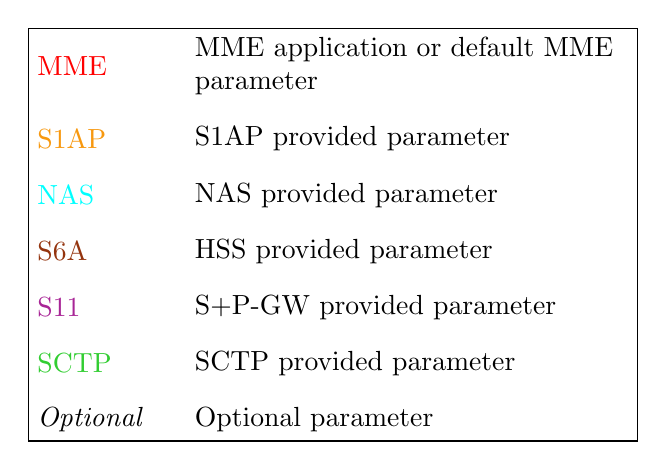
\begin{tikzpicture}
  \matrix (matrixl3) [square matrix] {
      \node[](l1) {\mmecolor{MME}};         & \node[](ct1) {MME application or default MME parameter};\\
      \node[](l2) {\soneapcolor{S1AP}};     & \node[](ct2) {S1AP provided parameter};\\
      \node[](l3) {\nascolor{NAS}};         & \node[](ct3) {NAS provided parameter};\\
      \node[](l4) {\ssixcolor{S6A}};        & \node[](ct4) {HSS provided parameter};\\
      \node[](l5) {\spappcolor{S11}};       & \node[](ct5) {S+P-GW provided parameter};\\
      \node[](l6) {\sctpcolor{SCTP}};       & \node[](ct6) {SCTP provided parameter};\\
      \node[](l7) {\emph{Optional}};        & \node[](ct7) {Optional parameter};\\
  };

  %   \node[draw,fit=(ct1)(l1)(ct2)(l2)(ct3)(l3)(l4)(ct4)(l5)(ct5)] {};
  %   \node[below = 0.5cm of l2](l3) {};
  %   \draw[below=0.5cm of l2, ->] (1,1) -- (0,1);
  \end{tikzpicture}
  \end{figure}
  \end{landscape}

  \begin{landscape}
\begin{figure}
  \begin{center}
  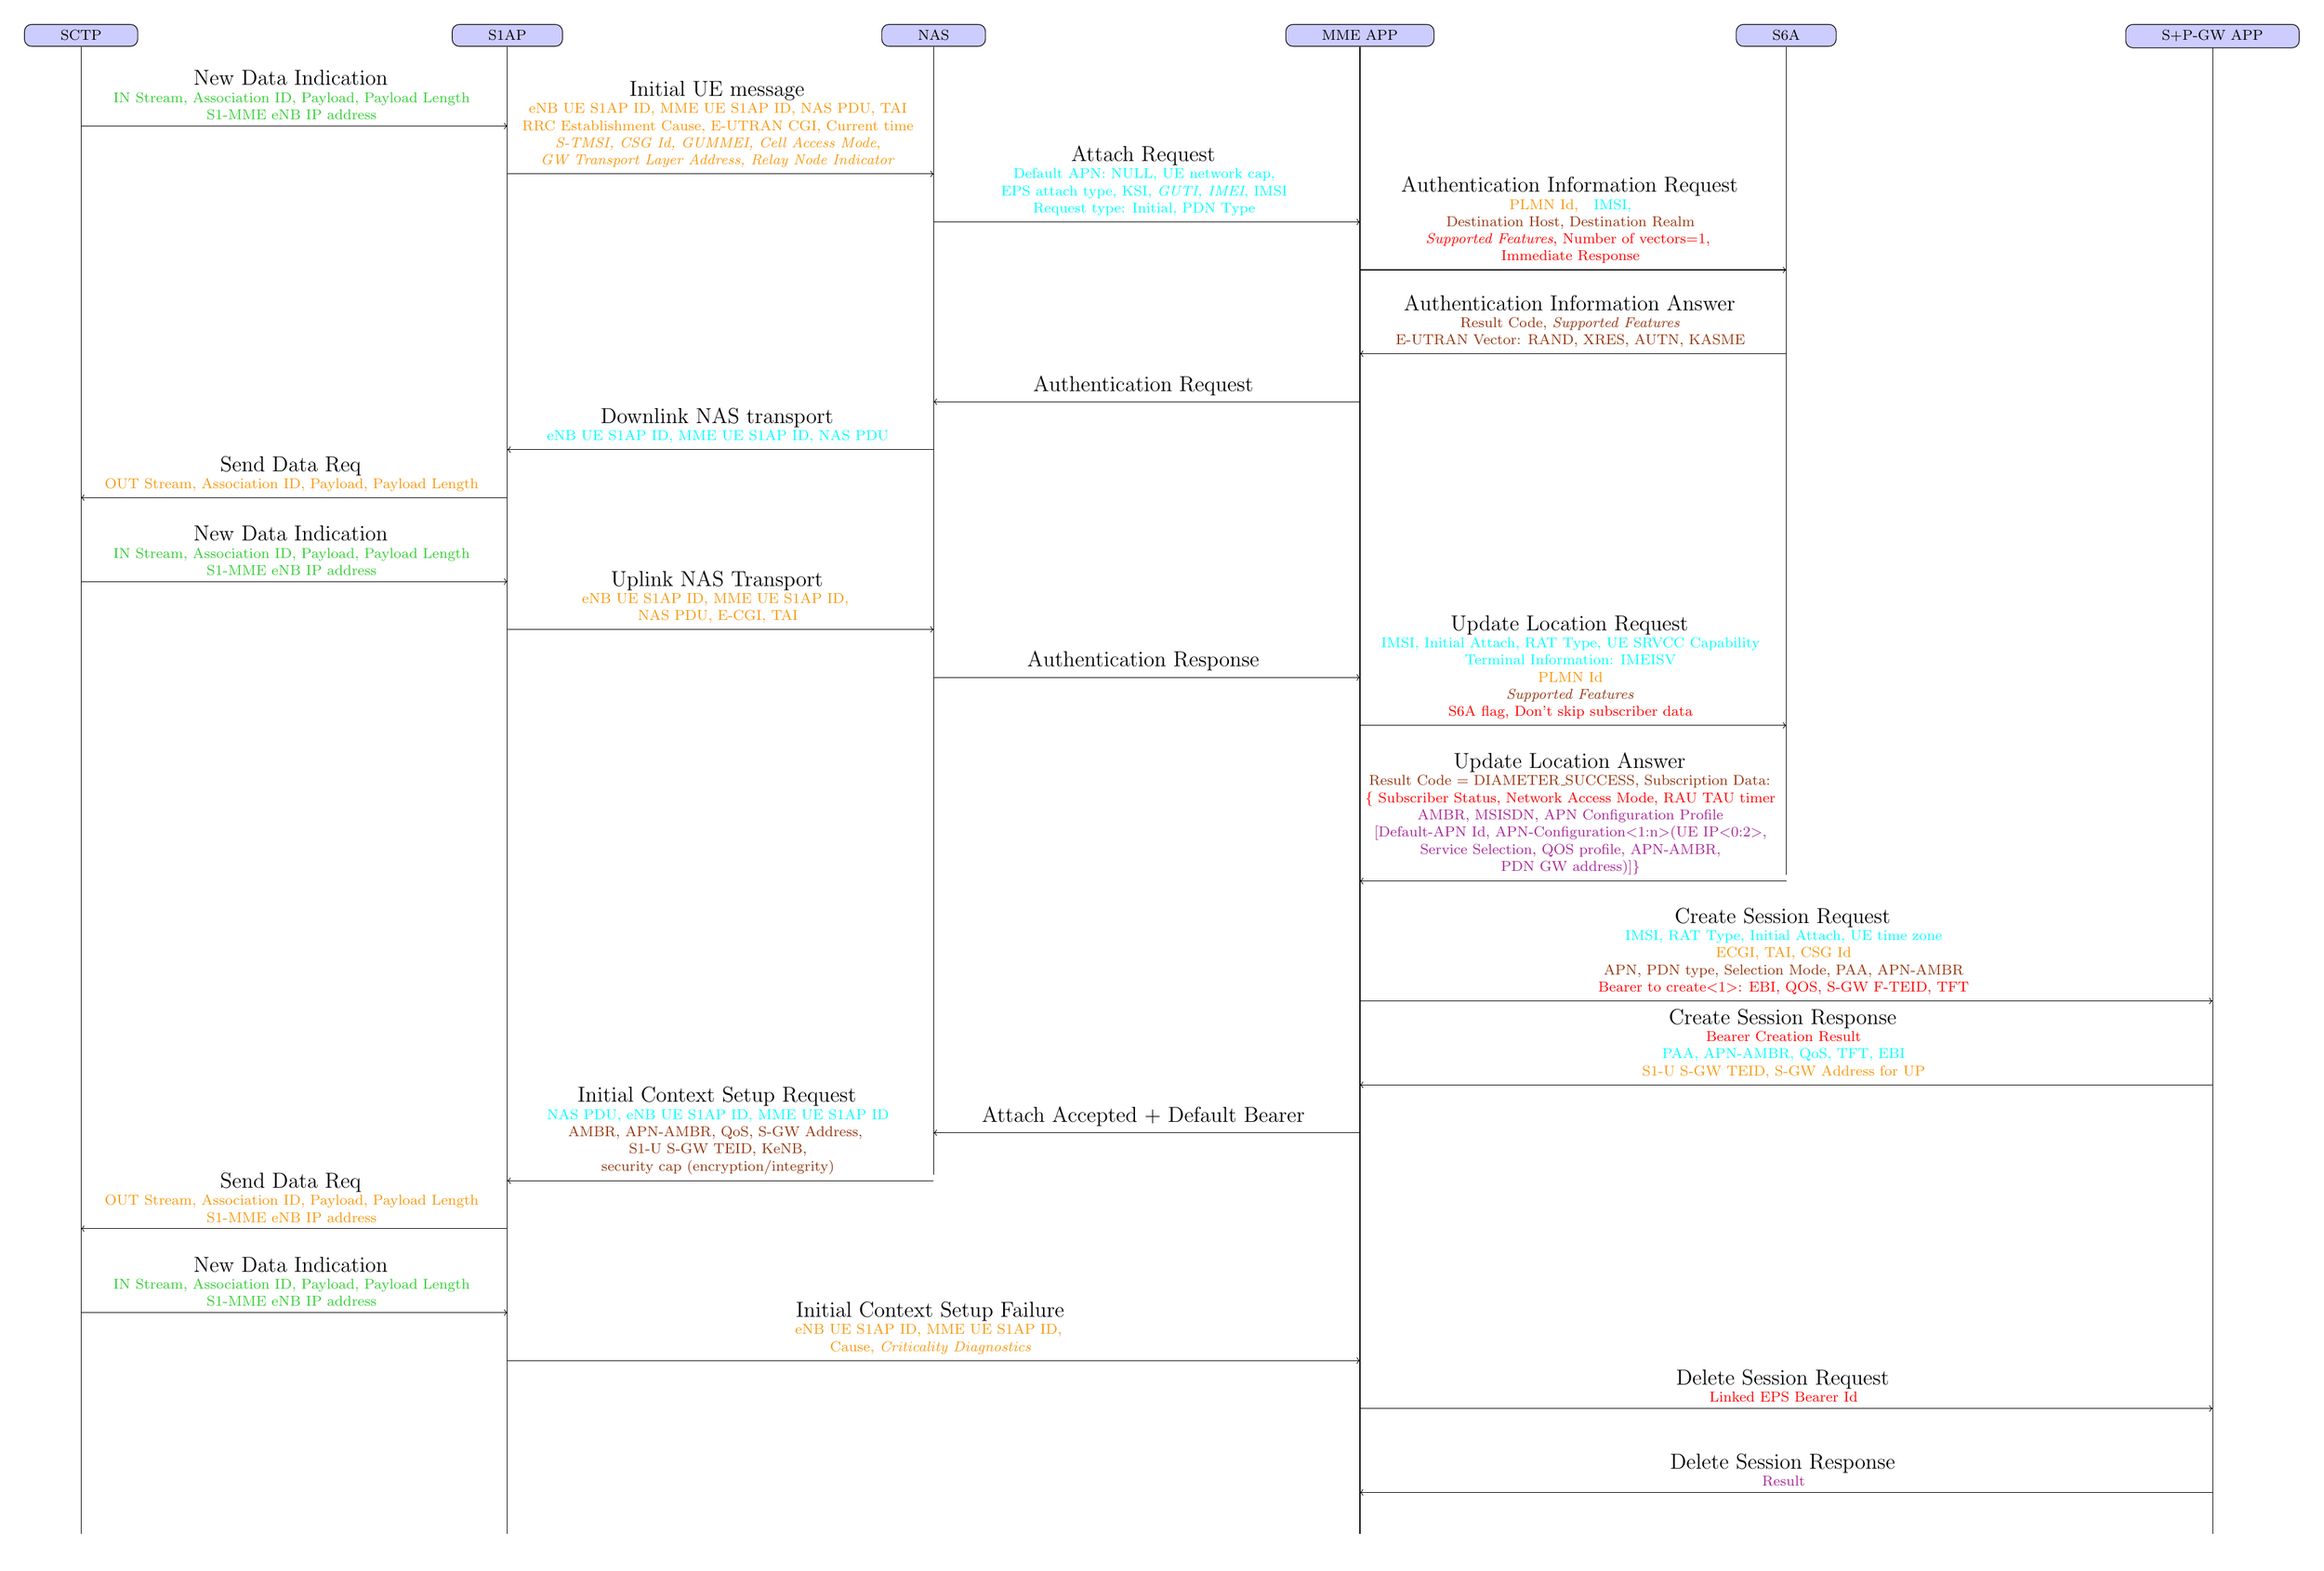
\begin{tikzpicture}
  \tikzstyle{every node}=[font=\footnotesize]
  \matrix (matrix6) [row sep=0.7cm, column sep={8.3cm,between origins}, matrix of nodes] {
      \node(SCTP) [schritt] {SCTP}; & \node(S1AP) [schritt] {S1AP};  & \node(NAS) [schritt] {NAS}; & \node(MMEAPP) [schritt] {MME APP}; & \node(S6A) [schritt] {S6A}; & \node(SPAPP) [schritt] {S+P-GW APP};\\\\
      \node(SCTP1) [] {}; & \node(S1AP1) [] {};\\
      & \node(S1AP2) [] {}; & \node(NAS1) [] {};\\
      & & \node(NAS2) [] {}; & \node(MMEAPP1) [] {};\\
      & & & \node(MMEAPP2) [] {}; & \node(S6A1) [] {};\\\\
      & & & \node(MMEAPP3) [] {}; & \node(S6A2) [] {};\\
      & & \node(NAS3) [] {}; & \node(MMEAPP4) [] {};\\
      & \node(S1AP3) [] {}; & \node(NAS4) [] {};\\
      \node(SCTP2) [] {}; & \node(S1AP4) [] {};\\\\
      \node(SCTP3) [] {}; & \node(S1AP5) [] {};\\
      & \node(S1AP6) [] {}; & \node(NAS5) [] {};\\
      & & \node(NAS6) [] {}; & \node(MMEAPP5) [] {};\\
      & & & \node(MMEAPP6) [] {}; & \node(S6A3) [] {};\\\\\\\\
      & & & \node(MMEAPP7) [] {}; & \node(S6A4) [] {};\\\\\\
      & & & \node(MMEAPP8) [] {}; & & \node(SPAPP1) [] {};\\\\
      & & & \node(MMEAPP9) [] {}; & & \node(SPAPP2) [] {};\\
      & & \node(NAS7) [] {}; & \node(MMEAPP10) [] {};\\
      & \node(S1AP7) [] {}; & \node(NAS8) [] {};\\
      \node(SCTP4) [] {}; & \node(S1AP8) [] {};\\\\
      \node(SCTP6) [] {}; & \node(S1AP11) [] {};\\
      & \node(S1AP12) [] {}; & & \node(MMEAPP12) [] {};\\
      & & & \node(MMEAPP13) [] {}; & & \node(SPAPP3) [] {};\\\\
      & & & \node(MMEAPP14) [] {}; & & \node(SPAPP4) [] {};\\
      \node(SCTPEND) [] {}; & \node(S1APEND) [] {}; & \node(NASEND) [] {}; & \node(MMEAPPEND) [] {}; & \node(S6AEND) [] {}; & \node(SPAPPEND) [] {};\\
  };

  \path[-]
  (SCTP)   edge (SCTPEND)
  (S1AP)   edge (S1APEND)
  (NAS)    edge (NAS8)
  (MMEAPP) edge (MMEAPPEND)
  (S6A)    edge (S6A4)
  (SPAPP)  edge (SPAPPEND)
  ;

  \draw[->] (node cs:name=SCTP1,anchor=center) -- node(arrow1)[above, align=center]{
      \commandname{New Data Indication}
      \\\sctpcolor{IN Stream, Association ID, Payload, Payload Length}
      \\\sctpcolor{S1-MME eNB IP address}}(node cs:name=S1AP1,anchor=center);
  \draw[->] (node cs:name=S1AP2,anchor=center) -- node(arrow2)[above, align=center]{
      \commandname{Initial UE message}
      \\\soneapcolor{eNB UE S1AP ID, MME UE S1AP ID, NAS PDU, TAI}
      \\\soneapcolor{RRC Establishment Cause, E-UTRAN CGI, Current time}
      \\\soneapcolor{\emph{S-TMSI, CSG Id, GUMMEI, Cell Access Mode},}
      \\\soneapcolor{\emph{GW Transport Layer Address, Relay Node Indicator}}}(node cs:name=NAS1,anchor=center);
  \draw[->] (node cs:name=NAS2,anchor=center) -- node(arrow3)[above, align=center]{
      \commandname{Attach Request}
      \\\nascolor{Default APN: NULL, UE network cap,}
      \\\nascolor{EPS attach type, KSI, \emph{GUTI, IMEI}, IMSI}
      \\\nascolor{Request type: Initial, PDN Type}}(node cs:name=MMEAPP1,anchor=center);
  \draw[->] (node cs:name=MMEAPP2,anchor=center) -- node(arrow4)[above, align=center]{
      \commandname{Authentication Information Request}
      \\\soneapcolor{PLMN Id, }\nascolor{IMSI,}
      \\\ssixcolor{Destination Host, Destination Realm}
      \\\mmecolor{\emph{Supported Features}, Number of vectors=1, }
      \\\mmecolor{Immediate Response}}(node cs:name=S6A1,anchor=center);
  \draw[->] (node cs:name=S6A2,anchor=center) -- node(arrow5)[above, align=center]{
      \commandname{Authentication Information Answer}
      \\\ssixcolor{Result Code, \emph{Supported Features}}
      \\\ssixcolor{E-UTRAN Vector: RAND, XRES, AUTN, KASME}}(node cs:name=MMEAPP3,anchor=center);
  \draw[->] (node cs:name=MMEAPP4,anchor=center) -- node(arrow6)[above, align=center]{
      \commandname{Authentication Request}}(node cs:name=NAS3,anchor=center);
  \draw[->] (node cs:name=NAS4,anchor=center) -- node(arrow7)[above, align=center]{
      \commandname{Downlink NAS transport}
      \\\nascolor{eNB UE S1AP ID, MME UE S1AP ID, NAS PDU}}(node cs:name=S1AP3,anchor=center);
  \draw[->] (node cs:name=S1AP4,anchor=center) -- node(arrow8)[above, align=center]{
      \commandname{Send Data Req}
      \\\soneapcolor{OUT Stream, Association ID, Payload, Payload Length}}(node cs:name=SCTP2,anchor=center);
  \draw[->] (node cs:name=SCTP3,anchor=center) -- node(arrow9)[above, align=center]{
      \commandname{New Data Indication}
      \\\sctpcolor{IN Stream, Association ID, Payload, Payload Length}
      \\\sctpcolor{S1-MME eNB IP address}}(node cs:name=S1AP5,anchor=center);
  \draw[->] (node cs:name=S1AP6,anchor=center) -- node(arrow10)[above, align=center]{
      \commandname{Uplink NAS Transport}
      \\\soneapcolor{eNB UE S1AP ID, MME UE S1AP ID, }
      \\\soneapcolor{NAS PDU, E-CGI, TAI}}(node cs:name=NAS5,anchor=center);
  \draw[->] (node cs:name=NAS6,anchor=center) -- node(arrow11)[above, align=center]{
      \commandname{Authentication Response}}(node cs:name=MMEAPP5,anchor=center);
  \draw[->] (node cs:name=MMEAPP6,anchor=center) -- node(arrow12)[above, align=center]{
      \commandname{Update Location Request}
      \\\nascolor{IMSI, Initial Attach, RAT Type, UE SRVCC Capability}
      \\\nascolor{Terminal Information: IMEISV}
      \\\soneapcolor{PLMN Id}
      \\\ssixcolor{\emph{Supported Features}}
      \\\mmecolor{S6A flag, Don't skip subscriber data}}(node cs:name=S6A3,anchor=center);
  \draw[->] (node cs:name=S6A4,anchor=center) -- node(arrow13)[above, align=center]{
      \commandname{Update Location Answer}
      \\\ssixcolor{Result Code = DIAMETER\_SUCCESS, Subscription Data:}
      \\\mmecolor{\{ Subscriber Status, Network Access Mode, RAU TAU timer}
      \\\spappcolor{AMBR, MSISDN, APN Configuration Profile}
      \\\spappcolor{[Default-APN Id, APN-Configuration$<$1:n$>$(UE IP$<$0:2$>$,}
      \\\spappcolor{Service Selection, QOS profile, APN-AMBR,}
      \\\spappcolor{PDN GW address)]\}}}(node cs:name=MMEAPP7,anchor=center);
  \draw[->] (node cs:name=MMEAPP8,anchor=center) -- node(arrow14)[above, align=center]{
      \commandname{Create Session Request}
      \\\nascolor{IMSI, RAT Type, Initial Attach, UE time zone}
      \\\soneapcolor{ECGI, TAI, CSG Id}
      \\\ssixcolor{APN, PDN type, Selection Mode, PAA, APN-AMBR}
      \\\mmecolor{Bearer to create$<$1$>$: EBI, QOS, S-GW F-TEID, TFT}}(node cs:name=SPAPP1,anchor=center);
  \draw[->] (node cs:name=SPAPP2,anchor=center) -- node(arrow15)[above, align=center]{
      \commandname{Create Session Response}
      \\\mmecolor{Bearer Creation Result}
      \\\nascolor{PAA, APN-AMBR, QoS, TFT, EBI}
      \\\soneapcolor{S1-U S-GW TEID, S-GW Address for UP}}(node cs:name=MMEAPP9,anchor=center);
  \draw[->] (node cs:name=MMEAPP10,anchor=center) -- node(arrow16)[above, align=center]{
      \commandname{Attach Accepted + Default Bearer}}(node cs:name=NAS7,anchor=center);
  \draw[->] (node cs:name=NAS8,anchor=center) -- node(arrow17)[above, align=center]{
      \commandname{Initial Context Setup Request}
      \\\nascolor{NAS PDU, eNB UE S1AP ID, MME UE S1AP ID}
      \\\ssixcolor{AMBR, APN-AMBR, QoS, S-GW Address, }
      \\\ssixcolor{S1-U S-GW TEID, KeNB,}
      \\\ssixcolor{security cap (encryption/integrity)}}(node cs:name=S1AP7,anchor=center);
  \draw[->] (node cs:name=S1AP8,anchor=center) -- node(arrow18)[above, align=center]{
      \commandname{Send Data Req}
      \\\soneapcolor{OUT Stream, Association ID, Payload, Payload Length}
      \\\soneapcolor{S1-MME eNB IP address}}(node cs:name=SCTP4,anchor=center);
  \draw[->] (node cs:name=SCTP6,anchor=center) -- node(arrow21)[above, align=center]{
      \commandname{New Data Indication}
      \\\sctpcolor{IN Stream, Association ID, Payload, Payload Length}
      \\\sctpcolor{S1-MME eNB IP address}}(node cs:name=S1AP11,anchor=center);
  \draw[->] (node cs:name=S1AP12,anchor=center) -- node(arrow22)[above, align=center]{
      \commandname{Initial Context Setup Failure}
      \\\soneapcolor{eNB UE S1AP ID, MME UE S1AP ID, }
      \\\soneapcolor{Cause, \emph{Criticality Diagnostics}}}(node cs:name=MMEAPP12,anchor=center);
  \draw[->] (node cs:name=MMEAPP13,anchor=center) -- node(arrow24)[above, align=center]{
      \commandname{Delete Session Request}
      \\\mmecolor{Linked EPS Bearer Id}}(node cs:name=SPAPP3,anchor=center);
  \draw[->] (node cs:name=SPAPP4,anchor=center) -- node(arrow25)[above, align=center]{
      \commandname{Delete Session Response}
      \\\spappcolor{Result}}(node cs:name=MMEAPP14,anchor=center);

  \end{tikzpicture}
  \end{center}
  \caption{MME detailed behaviour: Default Bearer Rejected (eNB Reject or Failure)} \label{fig:MME detailed behaviour: Default Bearer Rejected (eNB Reject or Failure)}

  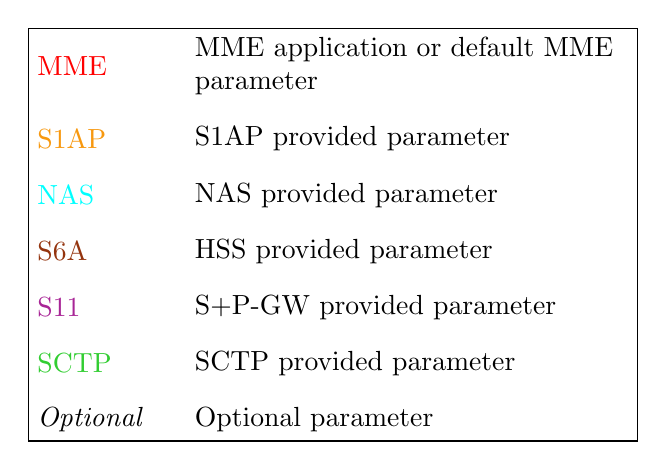
\begin{tikzpicture}
  \matrix (matrixl3) [square matrix] {
      \node[](l1) {\mmecolor{MME}};         & \node[](ct1) {MME application or default MME parameter};\\
      \node[](l2) {\soneapcolor{S1AP}};     & \node[](ct2) {S1AP provided parameter};\\
      \node[](l3) {\nascolor{NAS}};         & \node[](ct3) {NAS provided parameter};\\
      \node[](l4) {\ssixcolor{S6A}};        & \node[](ct4) {HSS provided parameter};\\
      \node[](l5) {\spappcolor{S11}};       & \node[](ct5) {S+P-GW provided parameter};\\
      \node[](l6) {\sctpcolor{SCTP}};       & \node[](ct6) {SCTP provided parameter};\\
      \node[](l7) {\emph{Optional}};        & \node[](ct7) {Optional parameter};\\
  };

  %   \node[draw,fit=(ct1)(l1)(ct2)(l2)(ct3)(l3)(l4)(ct4)(l5)(ct5)] {};
  %   \node[below = 0.5cm of l2](l3) {};
  %   \draw[below=0.5cm of l2, ->] (1,1) -- (0,1);
  \end{tikzpicture}
  \end{figure}
  \end{landscape}
\end{document}
